
\documentclass[12pt,twoside,openright]{report}
\usepackage[utf8]{inputenc}

% ---------- Necessary Packages ---------- %

% For equation Environtment
\usepackage{amsmath}

% Allows you to put figures. 
\usepackage{graphicx}
\usepackage{caption}
\usepackage{subcaption}

% Bibliography
\usepackage[sorting=none]{biblatex}
\addbibresource{references.bib}

% Colors
\usepackage{color}   % May be necessary if you want to color links

% Properly Formatted Units. 
\usepackage{siunitx}


% Footnote Package on image
\usepackage{fnpos}

% Intend after section title
\usepackage{indentfirst}

% Hyper links
\usepackage{hyperref}

\hypersetup{
    linktocpage=true,
    colorlinks=true,
    linkcolor=blue,
    filecolor=magenta,      
    urlcolor=cyan,
    citecolor=blue
    }




%  Abrebbiations. 

\newcommand{\hm}{$H^{-}$ }

% Formats the hole document
\usepackage[a4paper,width=150mm,top=25mm,bottom=25mm,bindingoffset=6mm]{geometry}

% Edits the headers and the footers. 
\usepackage{fancyhdr}

\def\vfootline{%
    \begingroup\color{black}\rule[-1mm]{0.4mm}{5mm}\endgroup}

% Fancy page style is for all the pages. 
\pagestyle{fancy}

\fancypagestyle{fancy}{%
    \fancyhf{}
    \fancyhead[ROH]{\slshape\nouppercase{\rightmark} \hspace{0.6cm} \vfootline \hspace{0.3cm}\thepage}
    \fancyhead[LEH]{\thepage \hspace{0.3cm} \vfootline \hspace{0.6cm} \slshape\nouppercase{\rightmark}}
}

% Plain page style is for apages with titles. 
\fancypagestyle{plain}{
  \fancyhf{}
  \fancyhead[ROH]{\vfootline \hspace{0.3cm}\thepage}
}

%\fancyfoot{}
%\fancyfoot[LE,RO]{\thepage}
%\fancyfoot[LO,CE]{Chapter \thechapter}

\renewcommand{\headrulewidth}{0.0pt}
%\renewcommand{\footrulewidth}{0.4pt}


% ----------- Necessary Paths ------------ %
\graphicspath{ {Figures/} }

% ----------------------------------------------------------------- %
% ----------------------------------------------------------------- %

\begin{document}


\begin{titlepage}
    \begin{center}
        
        \vspace*{1cm}
        \Huge
        \textbf{Thesis Title}
        
        \vspace{0.5cm}
        \LARGE
        Thesis Subtitle

        \vspace{1.5cm}

        \textbf{Araceli Navarro Fernandez}

        \vfill

        A thesis presented for the degree of \\
        Doctor of Philosophy

        \vspace{0.8cm}
        \large
        Department Name \\
        University Name \\
        Country \\
        Date


    \end{center}
\end{titlepage}

\pagestyle{plain}


\chapter*{Abstract} \label{Abstract}
\addcontentsline{toc}{chapter}{Abstract}

Summary about thesis....


\chapter*{Acknowledgements} \label{Acknowledgements}
\addcontentsline{toc}{chapter}{Acknowledgements}

asdasdasd

\tableofcontents
\addcontentsline{toc}{chapter}{Contents}


\listoffigures
\addcontentsline{toc}{chapter}{List of Figures}

\chapter*{List of Abbreviations}
\addcontentsline{toc}{chapter}{List of Abbreviations}

% ----------- INClude All the chapters ---------- %

\chapter*{Overview} \label{Overview}
\addcontentsline{toc}{chapter}{Overview}



\chapter{Overview} \label{ch:Overview}

\pagestyle{fancy}

\graphicspath{ {Figures/Chapter1_Overview/} }

\section{CERN accelerators complex}
\label{sec:CERN_acc_complex}

The European Organization for Nuclear Research (CERN) was founded in 1954, and it has become the largest particle physics laboratory in the world \parencite*[][]{ref:CernWebsite}. It sits astride the FrancoSwiss border near Geneva. It was one of Europe's first joint ventures and now has 23 member states. At CERN, the world's largest and most complex scientific instruments are used to study the basic constituents of matter, but the physics program at the laboratory is much broader, ranging from nuclear to high-energy physics, from studies of antimatter to the possible effects of cosmic rays on clouds.

CERN has not only provided advancements in fundamental sciences but has also pushed the frontiers of technology, with inventions such as the world wide web (www), Positron Emission Tomography (PET), etc. which have a positive impact on society globally.

CERN's accelerator complex (See \ref{fig:AccComplex} ) consists of many different types of linear and circular accelerators and interconnecting transfer lines to gradually accelerate the particles before injection into the Large Hadron Collider (LHC). 

Since 2020, Linear accelerator 4 (Linac4) became the source of proton beams for the LHC. Linac4 is an 86 \si{\meter} long machine. It accelerates negative hydrogen ions up to 160 \si{\mega \electronvolt}. The ions are then stripped of their two electrons during injection from Linac4 into the Proton Synchrotron Booster (PS Booster or PSB) to leave only protons. The PS Booster is made up of four superimposed synchrotron rings, with a 157 \si{\meter} circumference, which accelerates the injected protons up to 2 GeV for injection into the Proton Synchrotron (PS). 

Currently, the PS is the oldest accelerator in the chain. With a circumference of 628 meters, the PS operates up to 26 \si{\giga \electronvolt}. The Super Proton Synchrotron (SPS) is the second largest machine in the complex, measuring nearly 7 \si{\kilo \meter} in circumference. It takes the particles from the Proton Synchrotron and accelerates them up to 450 \si{\giga \electronvolt}. The CERN accelerator complex culminates with the Large Hadron Collider. The LHC consists of a 27 \si{\kilo \meter} ring of superconducting magnets, which guide two high-energy particle beams traveling in the opposite directions in separate beam pipes. The beams collide at four locations around the accelerator ring, corresponding to the positions of four particle detectors ATLAS, CMS, ALICE and LHCb. The High Luminosity Large Hadron Collider ( HiLumi LHC) project aims to deliver proton-proton collisions at 14 \si{\tera \electronvolt}.

\begin{figure}[h]
    \centering
    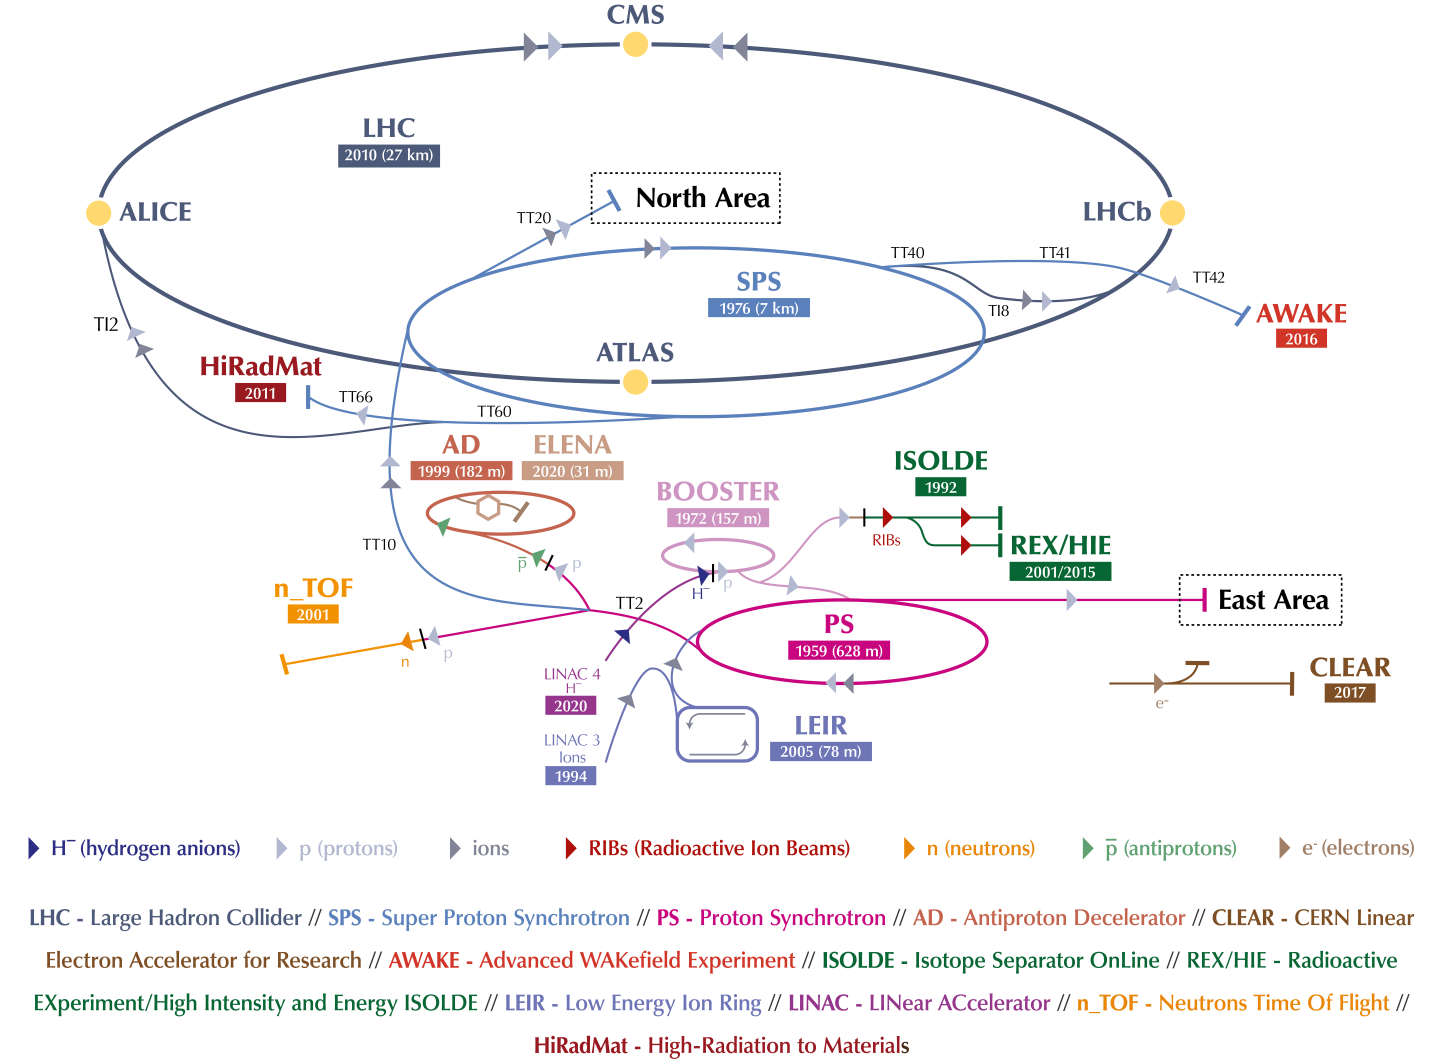
\includegraphics[width=0.95\columnwidth]{Figure_AcceleratorChain/cernComplex.png}
    \caption{CERN Accelerator Complex \parencite*[][]{ref:cerncomplex} . }
    \label{fig:AccComplex}
\end{figure}

Not only protons can be accelerated at the CERN accelerator complex. Linear accelerator 3 (Linac 3) is the starting point for the ions. It provides mainly lead ions, but also argon and xenon were used in the past. Experiments with oxygen are planned for the future. The long pulses of lead ions from Linac 3 are transformed into short, dense bunches by the Low Energy Ion Ring (LEIR) before they are injected into the PS. 

The injector chain apart from feeding the LHC is also used to deliver particles to several other experiments carried out at CERN, including Antimatter research on the Antiproton Decelerator (AD) and Extra Low ENergy Antiproton (ELENA), radioactive ion beam research on ISOLDE, research on neutron-nucleus interactions on the n-TOF facility, research on radiation-induced damage on materials in the HiRadMat facility and even studies on the use of proton-driven plasma wake-fields in AWAKE. 

\section{Linear Accelerator 4 (LINAC4)}
\label{sec:LINAC4}

As part of the LHC injection upgrade (LIU), CERN approved in 2007 the construction of LINAC4, to substitute the, by then existent, LINAC2 accelerator. The main goal for the construction of LINAC4 was to increase the beam brightness out of the PSB by a factor of 2, making possible an upgrade for the LHC injectors for higher intensity and eventually an increase of LHC luminosity \parencite*[]{ref:LIU}. 

The increase in beam brightness is achieved by combining two effects, the increase of the top energy to \SIlist[]{60}{\mega \electronvolt} (compared to the \SI[]{50}{\mega \electronvolt} given by LINAC2), which reduces significantly the space charge effect causing emittance blow up in the PSB. Secondly, the use of $H^{-}$ ions instead of protons makes it possible to inject into the PSB via the charge exchange scheme, which is explained in detail in Chapter \ref{ch:H0Hm}.

\begin{figure}[h]
    \centering
    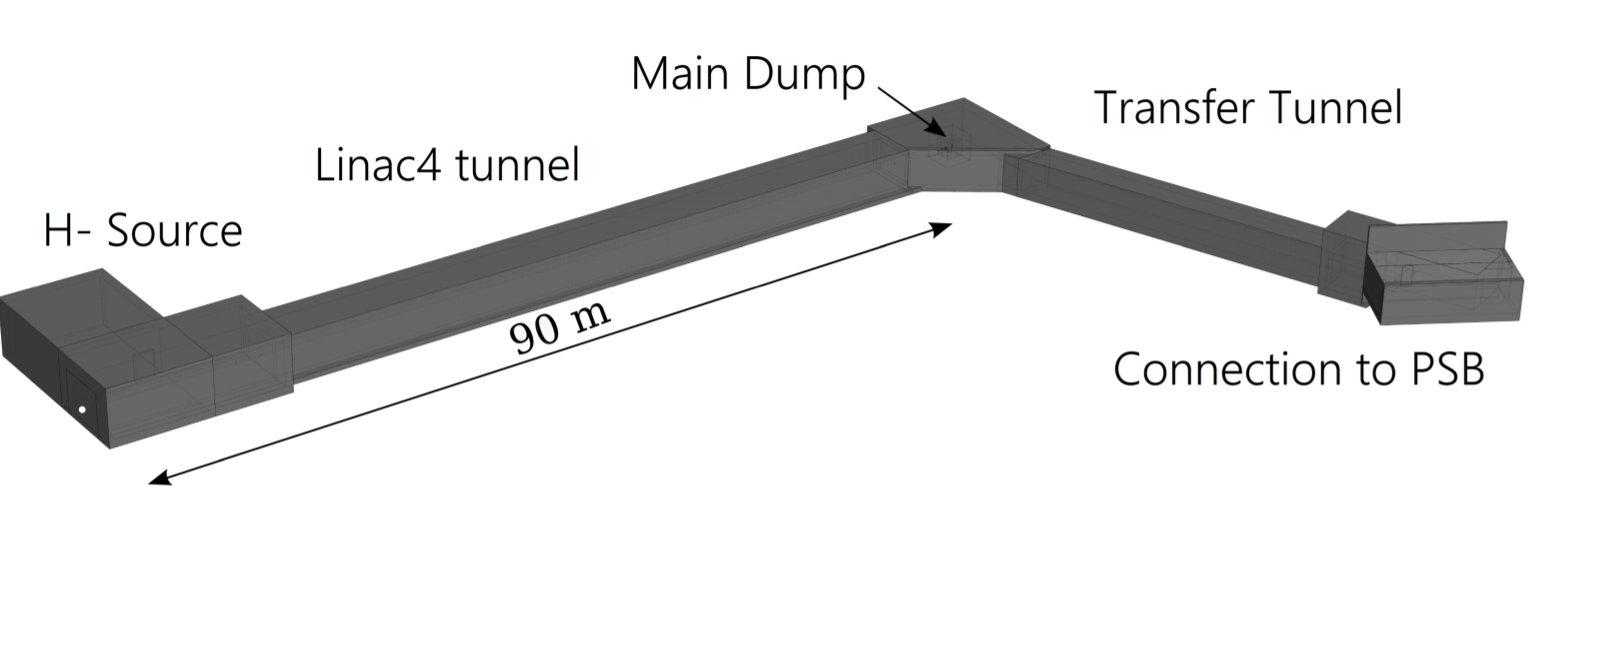
\includegraphics[width=0.70\columnwidth]{Linac4_Layout/linac4_Layout.png}
    \caption{General Layout of LINAC4 and its transfer-line to the PSB. }
    \label{fig:Linac4_layout}
\end{figure}

LINAC4 is \SI[]{86}{\metre} long and is located 12 m below ground. Figure \ref{fig:Linac4_layout} shows the source, tunnel, dump and transfer line to the PSB. Beams began to be produced in 2013 and the milestone energy of \SIlist[]{160}{\mega \electronvolt} was reached in 2016, after the commissioning of all the accelerating structures. During the long shut-down (2019-2020), LINAC4 finally replaced LINAC2 as the source of protons for the LHC. 

A more detailed description of the architecture of the accelerating section of LINAC4 is shown in figure \ref{fig:Linac4_acc}. The accelerating sequence is quite standard for a pulsed LINAC design. The LINAC4 source is a cesiated molybdenum-surface radio-frequency plasma ion source \parencite*[][]{ref:SourceCite}. This source can produce $H^{-}$ ion beams of up to 400\si[]{\micro \second} pulse length, 40\si[]{\milli \ampere} at a maximum revolution frequency of \SI[]{0.8}{\hertz}

\begin{figure}[h]
    \centering
    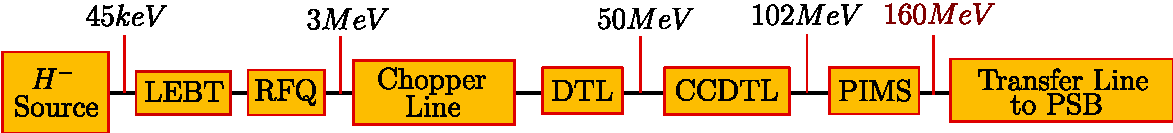
\includegraphics[width=1.0\columnwidth]{Linac4_AcceleratingPart/Linac4_acc.pdf}
    \caption{LINAC4 accelerating components layout. }
    \label{fig:Linac4_acc}
\end{figure}

The Low Energy Beam Transport (LEBT) line provides the beam matching from the source to the RFQ (Radio Frequency Quadrupoles) and contains the diagnostics to monitor the source. The three meter RFQ performs the beam capture and bunching and accelerates the particles to an energy of 3\si[]{\mega \electronvolt}. It is followed by a Medium Energy Beam Transport (MEBT) or "Chopper Line". This system consists of an electrostatic beam deflector followed by a beam dump. The purpose of this line is to avoid losses at higher energies when the induced radiation is higher. 

Three types of losses are treated with this system. Firstly, losses due to instable LINAC4 pulses. Secondly, it can be used to clean the first few tens of \si[]{\micro \second} of the beam pulse which are generally not stable. Finally, its purpose is to create "holes" in the beam pulse, timed with the rise-time of the PSB distributor, which switches the incoming LINAC4 beam between the four Booster Rings.  

The chopping line is followed by a series of three accelerating structures. The Drift Tube Linac (DTL) is divided in three tanks and accelerates the beam up to 50\si[]{\mega \electronvolt}. The Cell-Coupled Drift Tube Linac (CCDTL) is made of 7 accelerating modules for a top energy of 102 \si[]{\mega \electronvolt}. Finally, the Pi-Mode Structure (PIMS) brings the energy of the beam to the desired 160 \si[]{\mega\electronvolt}. More information about LINAC4 and its conforming parts can be found in \parencite*[]{ref:Linac4Technical}.  

In the current operational conditions, the LINAC4 pulse structure consists of four individual macro pulses, typically 20 - 100  \si[]{\micro \second}long (depending on the required number of injected turns per ring) and separated by a 1 \si[]{\micro \second} particle-free gap (See figure \ref{fig:Linac4PulseStruct}). Each macro-pulse consists of a train of 500 \si[]{\pico \second} long micro-bunches that are spaced by intervals of 2.8 \si[]{\nano \second} \parencite*[]{ref:Linac4PulseStruct}. In this document, we will focus on the beam pulse, that is, the convination of this four macro pulses.

\begin{figure}[h]
    \centering
    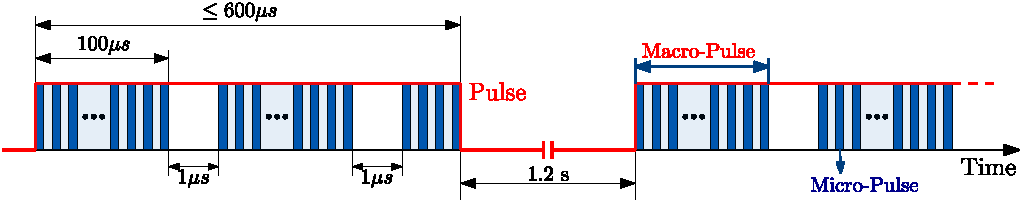
\includegraphics[width=1.0\columnwidth]{Figure_Linac4PulseStructure/Linac4_PulseStruct.pdf}
    \caption{LINAC4 Pulse Structure }
    \label{fig:Linac4PulseStruct}
\end{figure}


\section{Accelerator Physics Principles}
\label{sec:AccPhysPrinc}

The topic of Accelerator physics is very broad, in this section only an overview of the topics of interest for this document will be introduced. These topics include a quick overview of the basic concepts of beam dynamics, transverse plane, beam size and emittance. For a much more complete introduction to the world of accelerator check \parencite*[][]{ref:BookAccPhysics}.

\subsection{Principles of beam dynamics}
\label{subsec:PrincBeamDyn}

For describing the movement of the particles in an accelerator, the Frenet-Serret coordinate system, shown in figure \ref{fig:CoordinateSystem}, is commonly used. S defines the longitudinal coordinate and it is always tangent to the reference path. X and Y define the transverse plane (orthogonal to the particle trajectory). x(s) and y(s) describe the particle's deviation from the reference path at each point. $\rho(s)$ commonly defines the curvature of the reference orbit at each point. 


\begin{figure}[h]
    \centering
    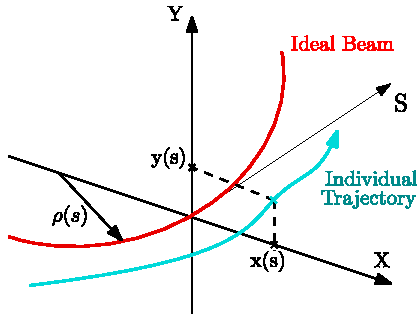
\includegraphics[width=0.5\columnwidth]{Figure_CoordinateSystem/CoordinateSystem.pdf}
    \caption{Frenet-Serret coordinate system.}
    \label{fig:CoordinateSystem}
\end{figure}

The theoretical conception of an accelerator starts by assuming constant energy and a stable beam trajectory. The scope of a particle accelerator design is to guide the beam of particles along the reference path and accelerate them to the desired energy. This is achieved by applying electromagnetic forces to the charged particles. Lorentz's law describes the force acting on a particle of charge "q" traveling in an electromagnetic field:

\begin{equation}
    \vec{F} = q \left( \vec{E} + \vec{v} \times  \vec{B}\right)
    \label{eq:LorentzLaw}
\end{equation}

Where $\vec{E}$ and $\vec{B}$ are the electric and magnetic fields and $\vec{v}$ is the particle velocity. Longitudinal electric fields accelerate the particles, while the transverse bending and focusing are provided by transverse magnetic fields. 

Particles which at the time $t_0$ have a non zero transverse coordinate $\left(x_0 , y_0 \right)$ and momentum $\left(x_{0}^{'} , y_{0}^{'} \right)$ start to perform oscillations in the horizontal and vertical planes,  called Betatron oscillations \parencite*[][]{ref:BookAccPhysics2}. These oscillations depend on the magnetic fields in the ring. The equation of motion on the transverse space can be derived from Lorentz's equation, and after some approximations it reads \parencite*[][]{ref:ApproxEqMotion}:

\begin{equation}
    \begin{aligned}
        x^{''} + \left(\frac{1}{\rho^{2}(s)}+\frac{1}{B\rho}\frac{\partial B_y(s)}{\partial x} \right)  x = 0 \\
        y^{''} - \frac{1}{B \rho}\frac{\partial B_y (s)}{\partial x}  y = 0
    \end{aligned}
    \label{eq:EqMotion}
\end{equation}


The product $B \rho$ is the magnetic rigidity and is equal to the ratio of the momentum to charge $p/q$. The only difference between the vertical and horizontal coordinates is the term $1/\rho^2(s)$ which is related to the centripetal force in the radial direction. These types of differential equations are often referred to as Hills equation \parencite*[][]{ref:HillEquation}, and describe a pseudo harmonic oscillator in which the spring constant depends on the position (s). For each element on the beamline, one can calculate the solution of the equation of motion. The solution of the equation can be expressed in a matrix formulation \parencite*[][]{ref:MatrixForm}:

\begin{equation}
    \begin{bmatrix}
        u(s) \\ u^{'}(s) 
   \end{bmatrix}
   = 
   \begin{bmatrix}
        C(s) & S(s) \\ C^{'}(s)  & S^{'}(s)
   \end{bmatrix}
   \begin{bmatrix}
        u_0 \\ u^{'}_0
   \end{bmatrix}
   =
   M(s) 
   \begin{bmatrix}
        u_0 \\ u^{'}_0
   \end{bmatrix}
\end{equation}

Where $M(s)$ is called the transformation matrix, which can be calculated individually for each type of beamline element. This matrix formalism is very useful as one can follow a particle trajectory along a complicated beam line by repeated matrix multiplication from element to element \parencite*[][]{ref:MatrixTransport}. Three commonly used transport matrices would be the following: 

\begin{itemize}
    \item Drift (no magnetic elements) of length L:
    
    \begin{equation}
        M_D
        =
        \begin{pmatrix}
             1 & L \\ 0 & 1
        \end{pmatrix}
    \end{equation}

    \item Focusing Quadrupole: 
    
    \begin{equation}
        M_{QF} =
        \begin{bmatrix}
             cos\left(\sqrt{k}L_Q\right) & \frac{1}{\sqrt{k}}sin\left(\sqrt{k}L_Q\right) \\
             -\sqrt{k}sin\left(\sqrt{k}L_Q\right) & cos\left(\sqrt{k}L_Q\right)
        \end{bmatrix}
    \end{equation}

    \item Defocusing Quadrupole:
    
    \begin{equation}
        M_{QD} =
        \begin{bmatrix}
             cosh\left(\sqrt{\left|k\right|}L_Q\right) & \frac{1}{\sqrt{\left|k\right|}}sinh\left(\sqrt{\left|k\right|}L_Q\right) \\
             -\sqrt{\left|k\right|}sinh\left(\sqrt{k}L_Q\right) & cosh\left(\sqrt{\left|k\right|}L_Q\right)
        \end{bmatrix}
    \end{equation}

\end{itemize}

In these equations, $L_Q$ refers to the length of the magnets and k is the effective focusing strength of the quadrupoles. 


\subsection{Particle beams and beam profile}
\label{subsec:TransBeamProf}

A beam or a bunch of particles is a collection of a very large number of particles whose center of gravity moves in a well-defined direction. If we consider the transverse plane X-Y (orthogonal to the beam direction of motion), one can obtain the particle distribution by noting the position of each particle that crosses this plane. If there is no coupling between the motion of the particles in the x and y directions, the distribution of the particles will be somehow elliptical, with the axis of the ellipse parallel to the x and y axes. See Figure \ref{fig:TransversePlane} for an example of transverse space particle distribution. 

\begin{figure}[h]
    \centering
    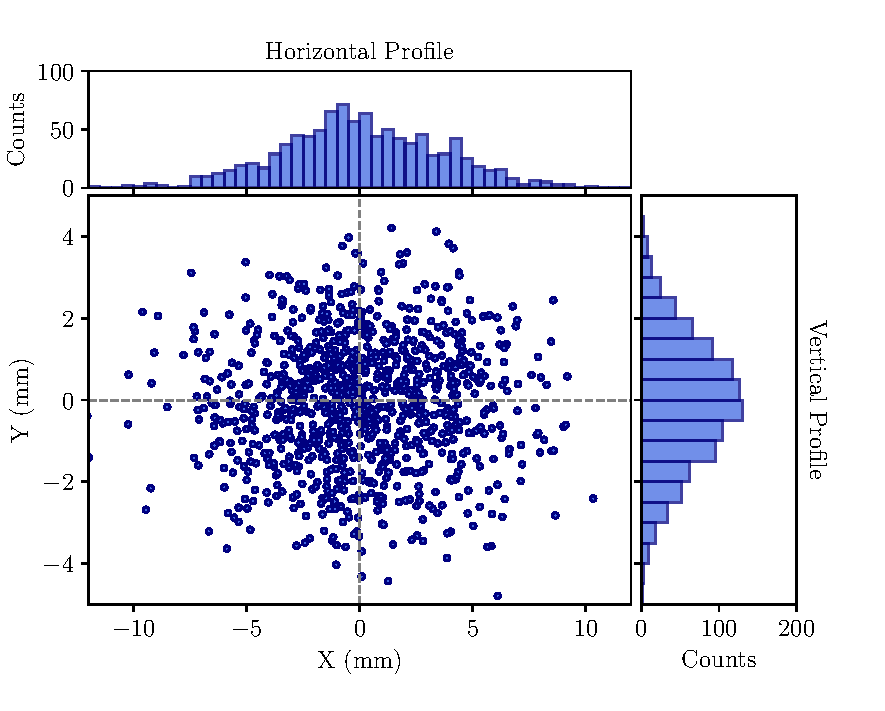
\includegraphics[width=0.9\columnwidth]{Figure_ParticlePositionExample/ParticlePosition.pdf}
    \caption{Example of Particle distribution in the X-Y space, with their corresponding projections.}
    \label{fig:TransversePlane}
\end{figure}

A histogram expressing the number of particles in a beam as a function of the transverse position is known as a beam profile. A Horizontal beam profile gives information about the number of particles at different x positions. A Vertical beam profile gives information about the number of particles at different y positions. 

A typical way of expressing the number of particles at a certain point in space is using a gaussian function:

\begin{equation}
    N(x,y) = \frac{N_{Tot}}{2\pi\sigma_x \sigma_y}\cdot exp\left(-\frac{1}{2}\left(\left(\frac{x-x_0}{\sigma_x}\right)^2 -\left(\frac{y-y_0}{\sigma_y}\right)^2\right)\right)
    \label{eq:GaussianDist}
\end{equation}

Here $x_0 , y_0$ are the coordinates of the center of the beam. $\sigma_x , \sigma_y$ are the standard deviation of the normally distributed beam of particles. $N_{Tot}$ refers to the total number of particles in the beam pulse. However, this expression is no more than an approximation, and one should be careful to understand its limitations. Usually, at the particle source, the beam of particles is far from Gaussian, but after some acceleration, this becomes a good approximation \parencite*[][]{ref:BookAccPhysics}.

\subsection{Transverse phase space}
\label{subsec:TransPhSp}

Each one of the particles in the beam will not only have a different position, but also a different direction of movement. The velocity vector of each particle can be decomposed into two components, one parallel to the beam direction (s) and one orthogonal to it (transverse velocity). The transverse velocity can then be discomposed into its components along the x-axis and y-axis. The phase space has information on both the position and the transverse velocity of each of the particles in the beam. Because the velocity and the momentum of the particles are related, one can express the information of the phase space in terms of the transverse momenta of the particles $\left(p_x , p_y \right)$. 

For convenience, the phase space is described by the transverse momentum $(p_x , p_y)$ normalized by the longitudinal momentum $(p_s)$. This quantities are expressed by: $x^{'} = p_x / p_s$ and $y^{'} = p_y / p_s$. For reprsenting the phase space, two charts are needed, one for the vertical plane and one for the horizontal plane. Figure \ref{fig:PhaseSpace} shows an example of particle distribution in the phase space. 

\begin{figure}[h]
    \centering
    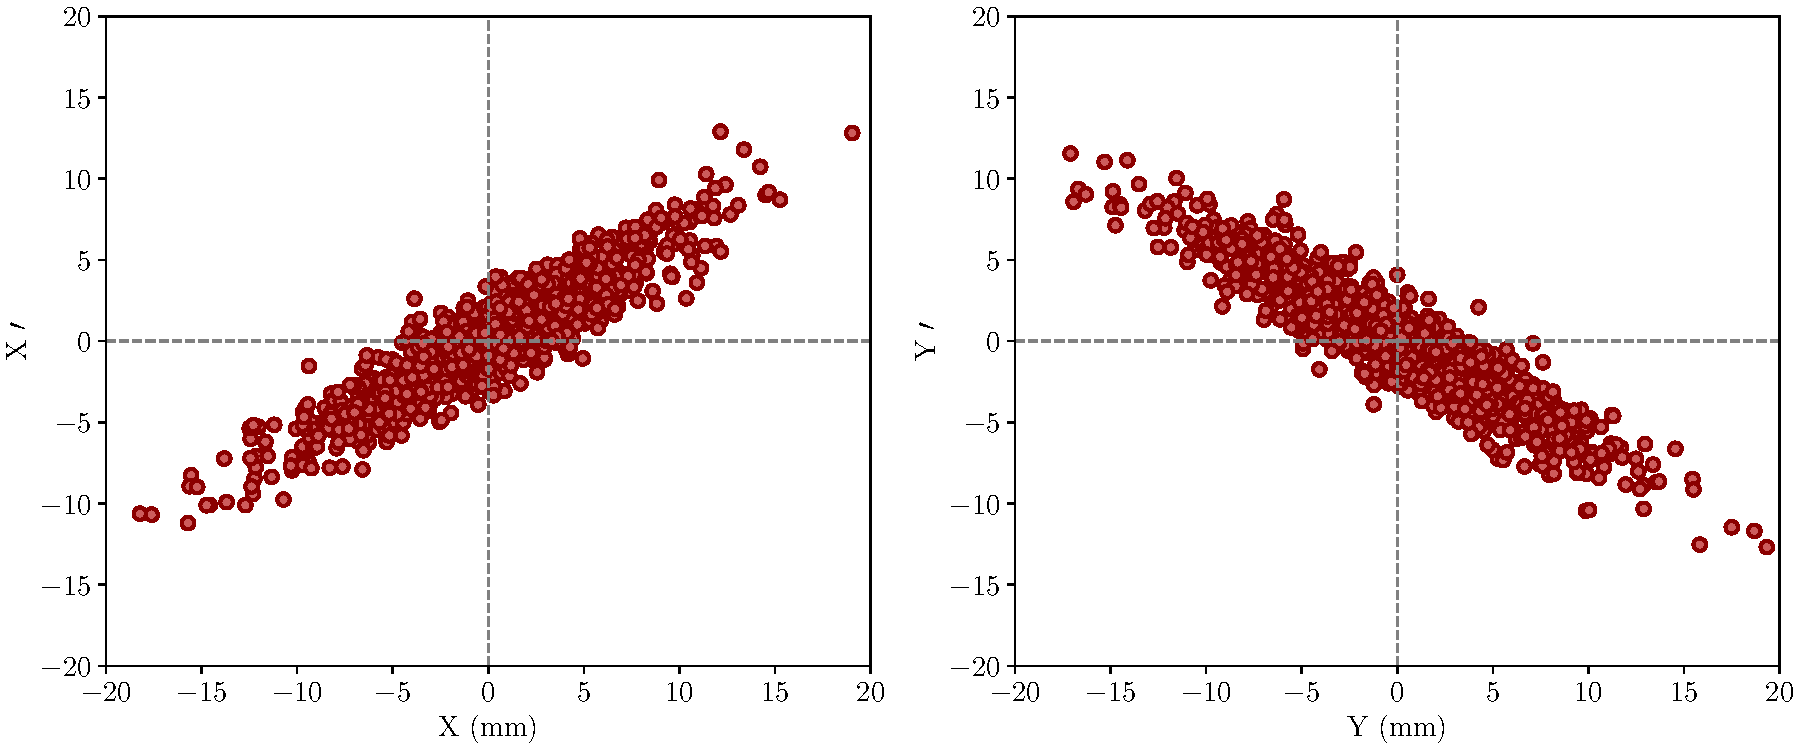
\includegraphics[width=1.0\columnwidth]{Figure_PhaseSpaceDist/PhaseSpaceDist.pdf}
    \caption{Particle distribution in the transverse phase space. }
    \label{fig:PhaseSpace}
\end{figure}

The particle distributions in the phase space are again ellipses, but in this case, they are tilted with respect to the axes. The phase space contains the whole description of the states of all the particles for a particular plane. This information is needed if one wants to calculate the subsequent motion of the particles in the electromagnetic fields of the accelerator. 

\subsection{Transverse beam emittance}
\label{subsec:TransBeamEm}

A formal description of the phase space can be developed by exploiting the elliptical shape of the phase space. The equation of the phase-space ellipse can be described as follows: 

\begin{equation}
    \epsilon = \gamma x^2 + 2\alpha x x^{'} + \beta x^{'2}
    \label{eq:ellipse}
\end{equation}

The parameters $\alpha, \beta, \gamma$ are referred to as the Courant-Synder parameters \parencite*[][]{ref:BookAccPhysics}. The area of the ellipse is simply $A = \pi \epsilon$. In the accelerator and beam physics language, the area in the phase space ($\epsilon$) containing the particles is called the emittance, statistical emittance, or more precisely it is called the rms-emittance. In the case of Gaussian beams, the concept of rms-emittance can be directly interpreted as the area containing a fraction (f) of ions. For example, it can be proven \parencite*[][]{ref:BookAccPhysics2},  that the curve of area $\epsilon$ should contain a $39\%$ of particles. Table \ref{tab:ParticleProportion} resumes the fraction of particles in a gaussian beam associated with various emittances. 


\begin{table}[h]
    \centering
    \begin{tabular}{cc}
    \hline
    Emittance $\epsilon(f)$ & Particle Fraction ($\%$) \\ \hline
    $\epsilon_{rms}$       & 15                     \\
    $\pi \cdot \epsilon_{rms}$     & 39                     \\
    $2\pi \cdot \epsilon_{rms}$  & 63                     \\
    $4\pi \cdot \epsilon_{rms}$  & 86                     \\
    $8\pi \cdot \epsilon_{rms}$   & 98                     \\ \hline
    \end{tabular}
    \caption{Fraction (f) of particles in a Gaussian beam associated with different definitions of emittance.}
    \label{tab:ParticleProportion}
\end{table}

\begin{figure}[h]
    \centering
    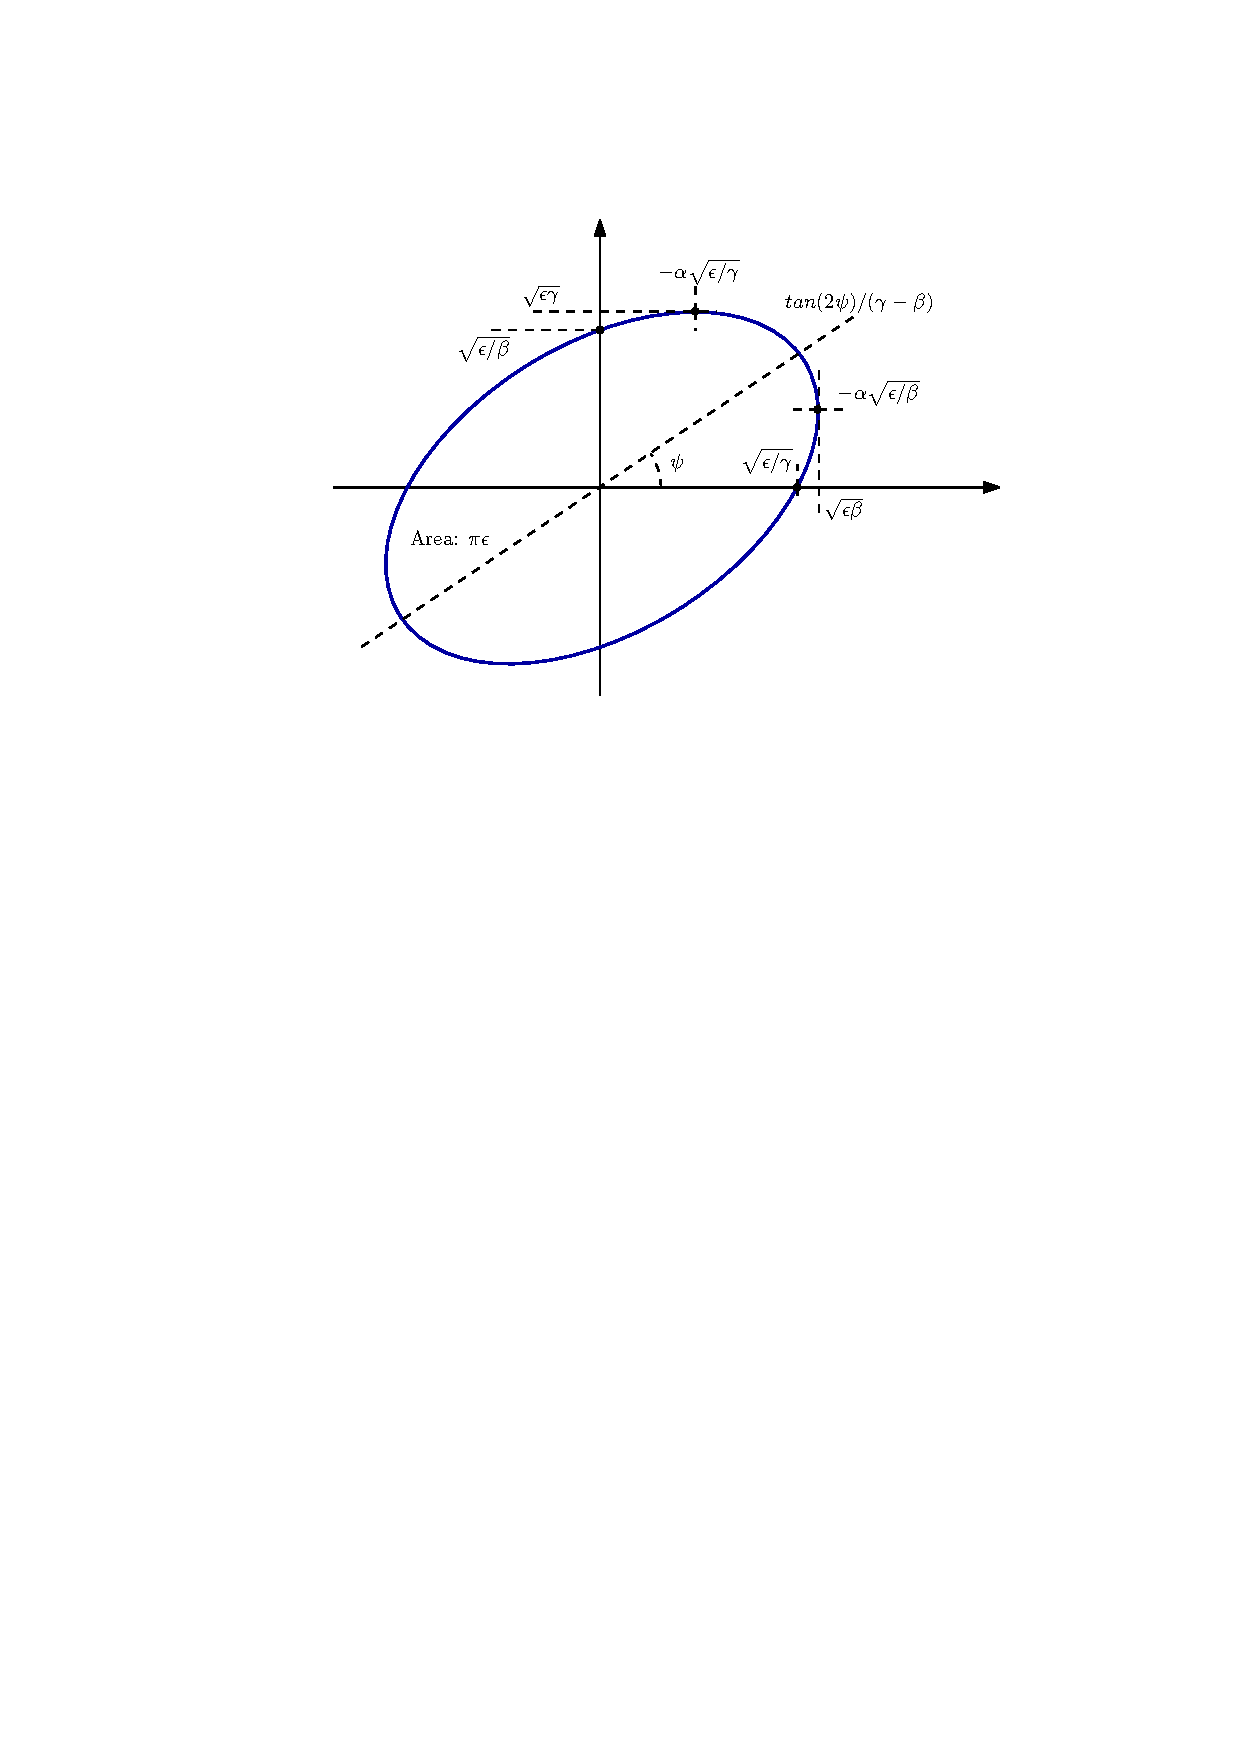
\includegraphics[width=0.7\columnwidth]{Figure_GeometricEmittance/GeometricEmittancve.pdf}
    \caption{Phase Space, geometrical ellipse. }
    \label{fig:CouranSnyder}
\end{figure}

    
Figure \ref{fig:CouranSnyder} shows a geometrical description of the Courant-Snyder parameters. These parameters $\left(\alpha , \beta , \gamma \right)$ are not independent, the third parameter is typically defined in therms of the other two: 

\begin{equation}
    \gamma = \frac{1 + \alpha^{2}}{\beta}
\end{equation}

Some other quantites, also very important for the understanding of the mathematical formulation of the transverse emittance are the following: 

\begin{equation}
    x_{rms}^2 = \left<x^2\right> =\frac{1}{N}\sum_{i=1}^N x_i^2
\end{equation}
\begin{equation}
    x_{rms}^{'2} = \left<x^{'2}\right> = \frac{1}{N}\sum_{i=1}^N x_i^{'2}
\end{equation}
\begin{equation}
    x x^{'}_{rms} =  \left< x x^{'}\right> = \frac{1}{N}\sum_{i = 1}^{N} x_{i} x^{'}_{i}
\end{equation}

With $x_{i} = X_{i} - \left< X \right>$ and $x^{'}_{i} = X_{i} - \left< X^{'}\right>$. $X_{i}$ and $X_{i}^{'}$ being the horizontal position and momentum of the individual particles conforming the beam. For convenience this parameters can be expressed in a matrixs form as follows: 

\begin{equation}
    \Sigma = 
    \begin{pmatrix}
        \left< x^{2} \right> & \left< x x^{'} \right> \\
        \left< x x^{'} \right> & \left< x^{' 2} \right>
    \end{pmatrix}
    = \epsilon 
    \begin{pmatrix}
        \beta & - \alpha \\ -\alpha  & \gamma
    \end{pmatrix}
\end{equation}

The rms-emittance ($\epsilon$) can also be obtained from this parameters as follows: 

\begin{equation}
    \epsilon = \pi \sqrt{\left<x^{2}\right>\left< x^{'2}\right> - '\left<x x^{'}\right>^{2}}
\end{equation}

\subsection{Phase Space Evolution}
\label{subsec:PhaseSpaceEvol}

In a transfer line or a storage ring (i.e. no acceleration), and assuming no energy losses due to radiation, Liouville's theorem establishes that emittance ( considering both transverse and longitudinal coordinates) is conserved \parencite*[][]{ref:EmittanceConserv}. However, the shape of the ellipse changes along the beam line. Figure \ref{fig:PhasSpaceEvol} illustrates a typical example of phase space evolution. 

\begin{figure}[h]
    \centering
    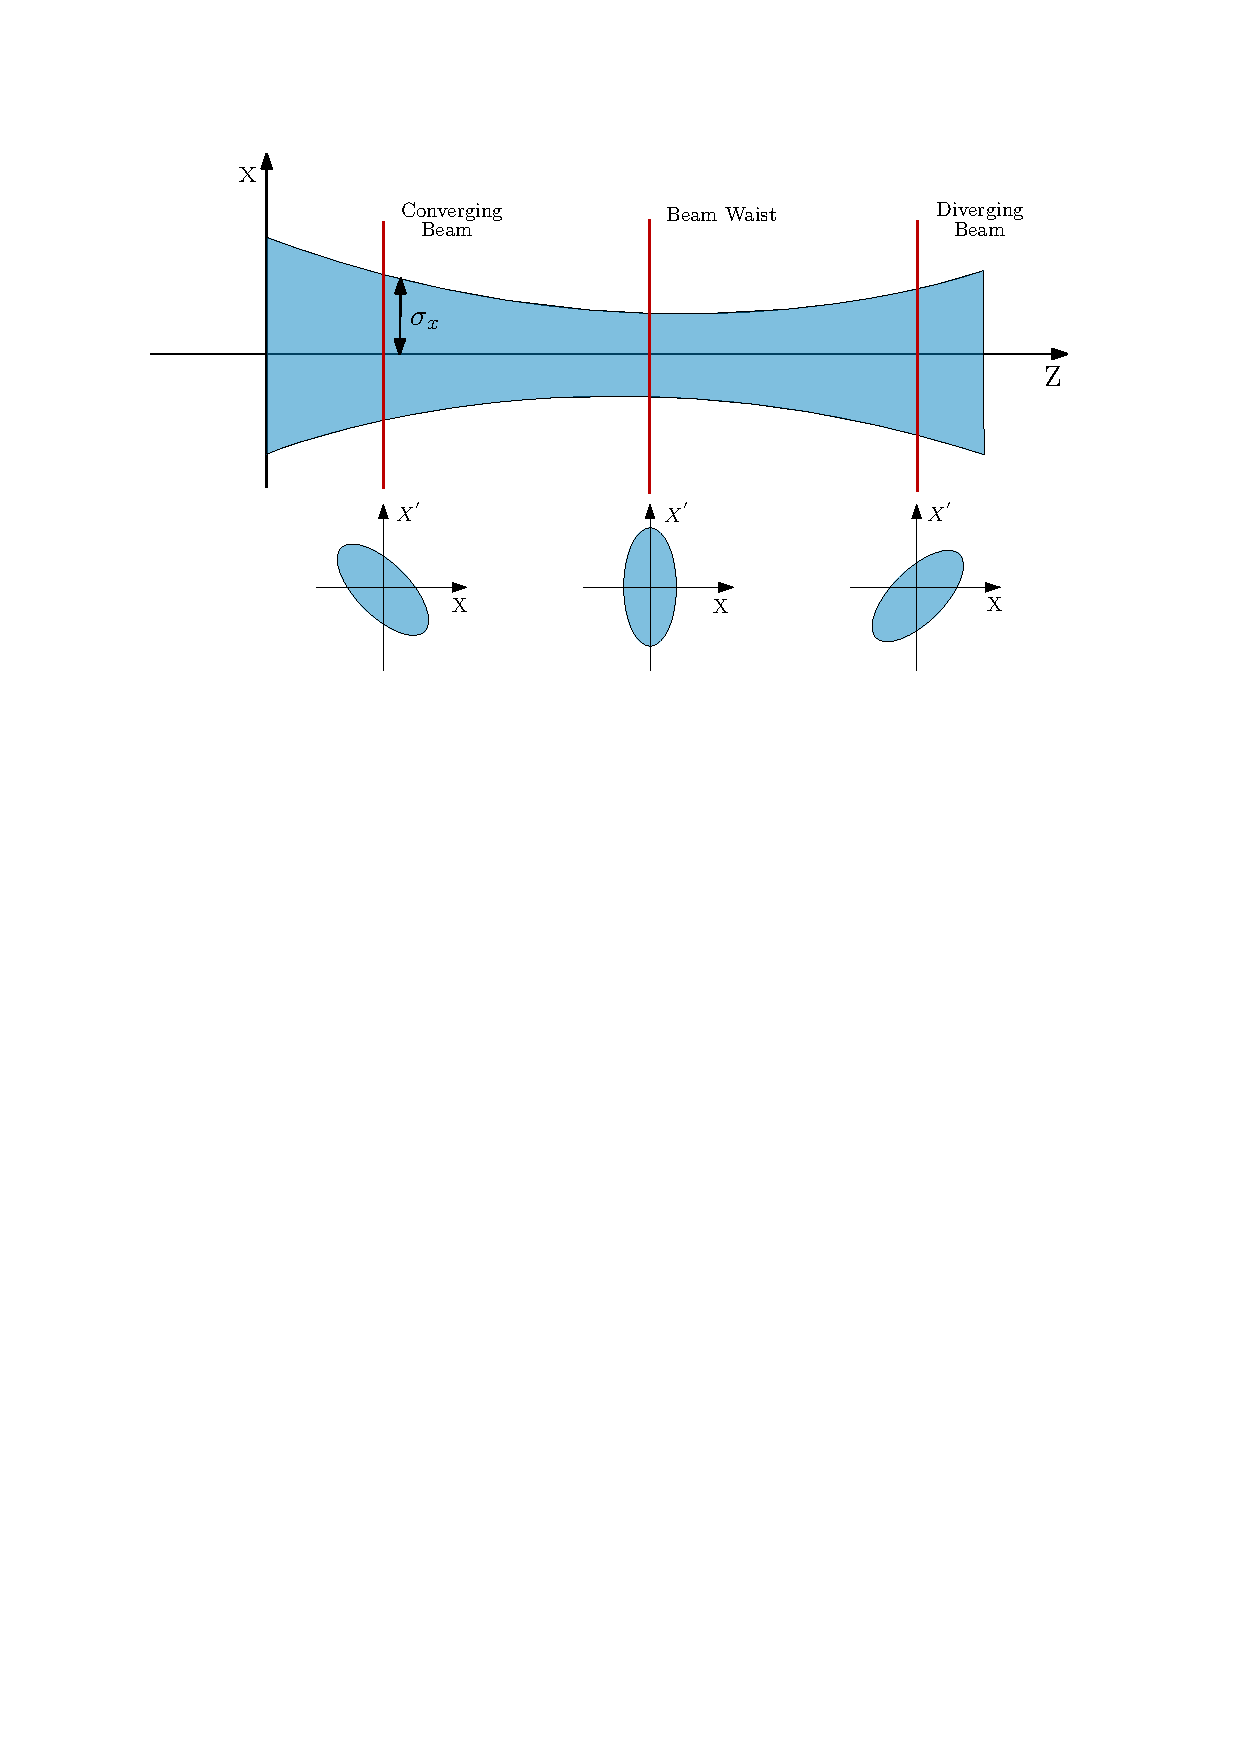
\includegraphics[width=0.9\columnwidth]{Figure_BeamEvolution/BeamEvolution.pdf}
    \caption{Example of phase space evolution. }
    \label{fig:PhasSpaceEvol}
\end{figure}

In the previous sections (Sec. \ref{subsec:PrincBeamDyn}) we saw how, in linear systems, points on the phase-space could be mapped from one location to the other through matrix multiplications. Similarly, assuming the following single-particle transport matrix:

\begin{equation}
    \begin{bmatrix}
         x_1 \\ x_1^{'} 
    \end{bmatrix}
    = 
    \begin{bmatrix}
       c & s \\ c^{'} & s^{'}
     \end{bmatrix}
     \begin{bmatrix}
        x_0 \\ x_0^{'}
     \end{bmatrix}
\end{equation}

After some algebraic calculations, one can obtain the following transport matrix for the Twiss parameters \parencite*[][]{ref:MatrixToTwiss}:

\begin{equation}
    \begin{bmatrix}
       \beta_1 \\ \alpha_1 \\ \gamma_1
    \end{bmatrix}
    =
\begin{bmatrix}
   c^2 & - c s & s^2 \\ -c c^{'} & cs^{'} + c^{'}s & -s s^{'} \\ c^{'2} & -2c^{'}s^{'} & s^{'2}
\end{bmatrix}
=
\begin{bmatrix}
   \beta_0 \\ \alpha_0 \\ \gamma_0
\end{bmatrix}
\label{eq:MatrixEq}
\end{equation}




\chapter{Beam Diagnostics} \label{ch:BeamDiagnostics}

\pagestyle{fancy}

\graphicspath{ {Figures/Chapter2_BeamInstrumentation/} }

Beam diagnostics and instrumentation are essential constituents of any particle accelerator. They allow us to monitor the behavior and properties of the particle beam. Without adequate diagnostics, one would be blindly operating an accelerator and it would be impossible to assess problems and improve performances. Different accelerator types require different diagnostics. Similarly, different beam properties require very different instrumentation systems and techniques.  \parencite*[][]{ref:BeamInstrumentationBook}, \parencite*[][]{ref:NotesBeamInst} and \parencite*[][]{ref:CASbeamInst}, are very recommendable references, where the topic of beam instrumentation is covered extensively but yet with a very accessible approach. 

This chapter will focus on describing the principles of some commonly used devices that will be of great relevance for understanding the concepts of this work. We shall focus on the measurements of two beam properties: 

\begin{itemize}
    \item Transverse Beam Profile Measurements: They allow the measurement of the transverse distribution of the particles throughout the accelerator. This measurement is important to control the beam width and position, as well as the transverse matching between different parts of the accelerator facility. In particular, we will focus on Secondary Emission Grids (SEM Grids) and Wire Scanners. 
    \item Beam Intensity Measurements: They allow to measure the total electrical current of the beam, which is one of the most important parameters for the operation of a particle accelerator. Current measurements allow, for example, to determine the transfer efficiencies in linacs and transfer lines. In this case, we will talk about Beam Current Transformers (BCT) and Faraday Cups (FC).
\end{itemize}

\section{Seconday Emission Grids (SEM Grids)}
\label{sec:SEMgrids}

Wire Grids or Secondary Electron EMission grids (SEM Grid) are devices composed of a large number of parallel fixed wires or strips. Figure \ref{fig:SEMgrid} shows an example of a SEM grid detector. They are interceptive devices, during the measurements, each one of the wires interacts directly with the beam of particles. During this process a current, proportional to the number of particles, is generated in each wire.  By measuring the current in all the wires a beam profile can be reconstructed. More detailed explanations about the current generation process and the profile reconstruction will be given in Chapters \ref{ch:BeamMatterInter} and \ref{ch:CurrentModeling}.

\begin{figure}[h]
    \centering
    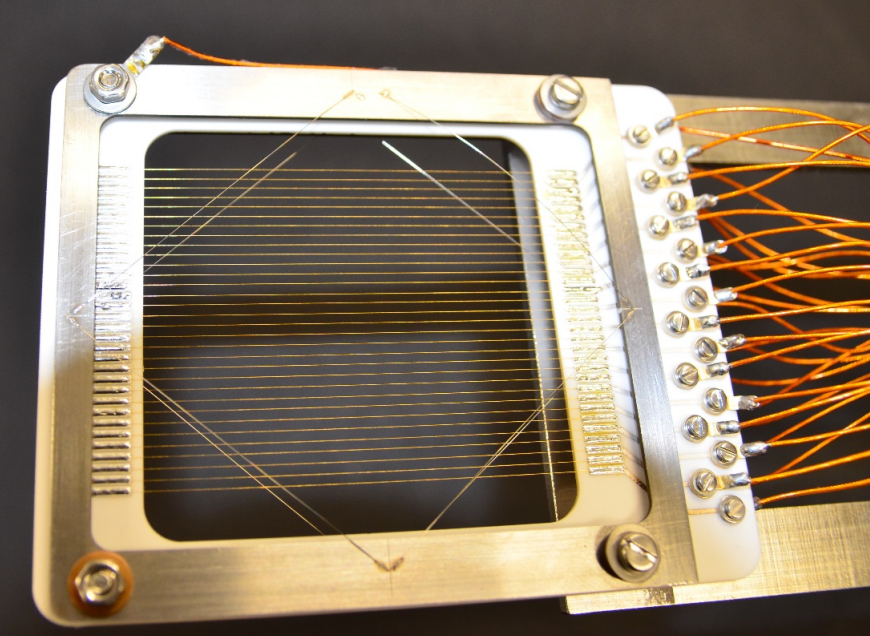
\includegraphics[width=0.6\columnwidth]{SEMGrid/semgrid.png}
    \caption{Example of a SEM grid installed at CERN accelerator Complex. }
    \label{fig:SEMgrid}
\end{figure}

SEM grids allow for a single-shot acquisition, and in some cases, it is possible to observe the evolution of the beam profile in the same pulse. The number of wires and the spacing between them varies from system to system. It is important for the detector to cover the whole range of the beam size and to have enough resolution to properly reconstruct the beam profile. Theoretically, a bigger detector with a larger number of wires would be more convenient. However, a system with too many wires implies an overly complicated acquisition system, it increases the probability of wire cross-talk and augments the construction costs. 

A typical number of wires ranges from 16 to 48. In some devices, the wires are spaced unevenly, with a denser distribution in the center. The diameter-to-spacing of the wires determines the attenuation of the beam current, which becomes an important parameter to consider for particles at low energies as they are fully stopped in the detector's material. It is common to consider that a $10 \%$ of the beam area is covered with the wires. 

The wire materials are selected to optimize signal generation and ensure proper thermal performance. Typical materials used for wire grid designs are Tungsten, Carbon (Graphite, CNT) or Titanium. The motion control of SEM grids is relatively simple, they are either fully inserted or fully retracted, and sometimes they might even be permanently positioned in the beam pipe with no motion control at all. 


\begin{figure}[h]
    \centering
    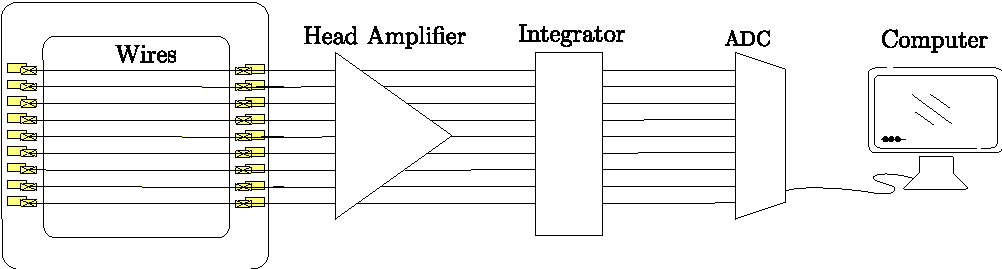
\includegraphics[width=1.0\columnwidth]{SEMgridDataADq/SEMdataAdc.pdf}
    \caption{Schematic representation of SEM Grid Adquisition system. }
    \label{fig:SEMGridReadOutSystem}
\end{figure}

Typically, the data acquisition chain is composed of a head amplifier that sits as near as possible to the grid, often in an area with radiation. It is followed by an integrator or signal conditioning circuit that sits away in a safe room. From the integrator, the signal is fed to a computer controller ADC. This scheme requires one signal cable per wire over the distance from the device to the ADC. 

The main drawbacks of this diagnostics device are the limit on the spatial resolution (which can be hardly reduced to less than a few hundred micrometers), the small wire signals and the complicated data adquisition system. 

\section{Wire Scanners}
\label{sec:WireScan}

Instead of using several wires with individual, expensive electronics, the Wire Scanners consist of a single wire that can be swept through the beam pipe (See figure \ref{fig:WireScan}). The main advantage of this technique is the high resolution that can be accomplished (sub-mm range). It is often used in accelerators with small beam sizes. These devices also intercept the beam of particles, however, its effect is practically negligible.

\begin{figure}[h]
    \centering
    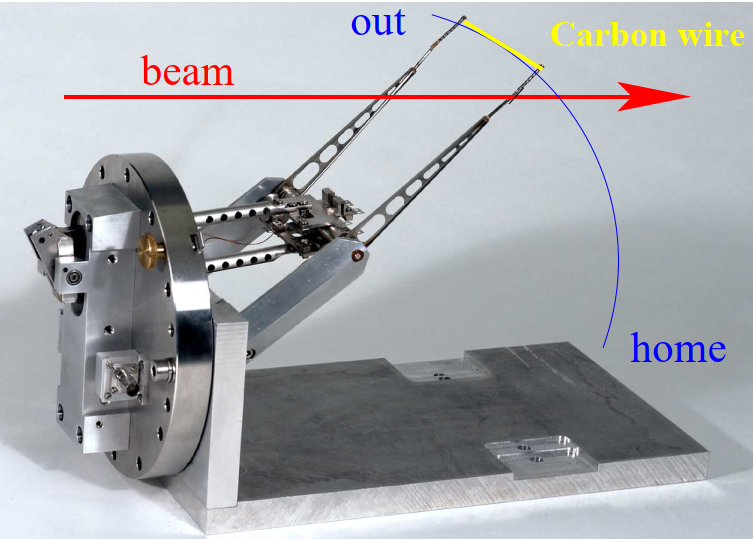
\includegraphics[width=0.6\columnwidth]{WireScanner/WireScanner.png}
    \caption{Rotational Fast Wire Scanner, used at CERN SPS. }
    \label{fig:WireScan}
\end{figure}

In the context of this thesis, we differentiate between two types of wire scanners:

\begin{enumerate}
    \item Slow Wire Scanners: They are commonly used on LINACs or transfer lines. Where the beam energy of the particle beam is small and the pulse structure consists of short pulses and low repetition rates. In this case, the profile is reconstructed by using the current generated in the detector by its interaction with the beam of particles. This signal is typically small and requires careful care in the acquisition. Usually, due to the low repetition rate of the beam in those areas, one sample is taken on each beam pulse, leaving plenty of time to move the wire from one pulse to the rest. 
    \item Fast Wire Scanners: For high energy and high repetition range beams, the profile is reconstructed by measuring a shower of secondary particles generated during the beam/wire interaction. These secondary particles might be hadrons (for proton/heavy ion accelerators) or photons (for electrons accelerators).  The secondary shower is detected outside the beam pipe, with a photo-multiplier tube. The speed of the wire movement varies over a very large range that can go from 1 \si[]{\metre /\second} up to 20 \si[]{\meter /\second}. In this case, the signal measured is typically quite large, due to the high photomultiplier range.  
\end{enumerate}

In both cases, the measurement of the wire position is a crucial aspect of the measurement, as the beam profile is reconstructed by correlating the wire position with the generated signal. The precision of the measurements of the wire scanner positions will therefore be a crucial factor in the measurement precision and resolution. In the case of fast wire scanners, the deformations or vibrations in the wire can also restrict the spatial resolution. Beam position and beam size variations during the measurement period can induce additional errors. 

For both, slow and fast wire scanners, the dimensions of the wire have a direct impact on the signal strengths and the measurement accuracy. In general beam sizes between 10 \si[]{\micro \metre} to 50 \si[]{\micro \metre}  are used.

\section{Beam Current Transformer (BCT)}
\label{sec:BCT}

An electric current flowing through a conductor gives rise to a magnetic field around the conductor, and passing a conducting loop through a magnetic field induces a current through the loop. These well-known principles of induction are used in the Beam Current Transformer (BCT). In this case, the particle beam is the primary current and can be described as: 

\begin{equation}
    I_{beam} = \frac{q e N_{part}}{t}
\end{equation}

Where $N_{part}$ is the number of particles of charge $q$ per unit time $t$. $e$ is the electron charge. This beam current generates a magnetic field as it travels through the accelerator. This magnetic field can be measured by placing a torus with high permeability around the beam. Some windings are placed around the tourus and then connected to an electrical circuit for read-out. Figure \ref{fig:BCTschema} shows a schematic representation of a BCT design. Measuring small beam currents becomes very challenging with these devices.

\begin{figure}[h]
    \centering
    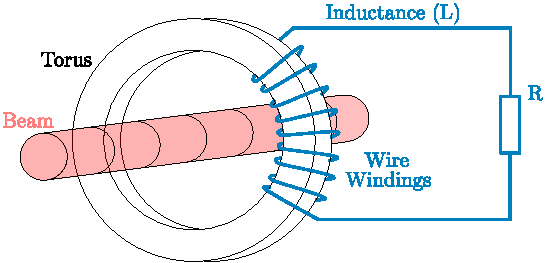
\includegraphics[width=0.6\columnwidth]{BCTschema/BCTschema.pdf}
    \caption{Schema of a current transformer built as a ring-core (torus). }
    \label{fig:BCTschema}
\end{figure}

\section{Faraday Cup (FC)}
\label{sec:FC}

A faraday cup (FC) is a beam stopper that measures the electrical current of the beam. A basic cup design is shown in figure \ref{fig:FaradayCup}. With a Faraday cup, a much lower current can be measured compared to a BCT, of the order of the \si[]{\pico \ampere} for low noise systems. These devices consist of an isolated metal cup connected to a current-sensitive pre amplifier. The current in these detectors is generated by measuring the total charge from the beam of particles that is deposited in them. High energetic particles not depositing all their energy in the detector material can affect negatively the measurement results. Similarly, a Secondary Electron (SE) suppression system has to be included in these devices to avoid errors in the current measurements. This is done by creating very long cups, high voltage suppression close to the entrance or by using a magnetic field. 

\begin{figure}[h]
    \centering
    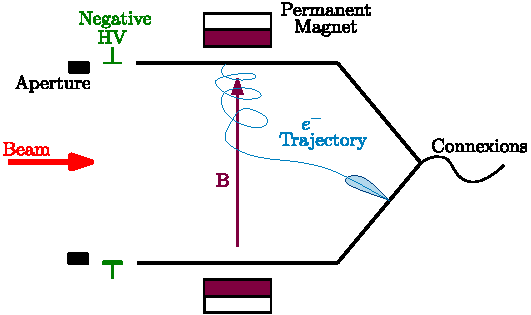
\includegraphics[width=0.6\columnwidth]{FCschema/FCschema.pdf}
    \caption{Schematic Representation of Faraday Cup. }
    \label{fig:FaradayCup}
\end{figure}

Sometimes, Faraday cups are also used for higher beam currents, where measurements with BCTs are also possible as they are easier to implement. In addition, cups serve as beam dumps. For high beam energies, one has to be concerned about the high thermal and structural shocks that these devices might suffer.

\section{Beam Intensity and Profile Measurements at CERN LINAC4.}

In this section, we will briefly show how the instruments just presented are used at CERN, LINAC4. All the results presented in this section correspond to the first profile and current measurements for the LBE run, which took place in November 2019 \parencite*[][]{ref:PresentationLBERun}. The objective of these measurements was to study the transverse profile evolution of the particle beam along the LINAC4 accelerator. 

Figure \ref{fig:Linac4Layout} shows a schematic representation of LINAC4 with the different detectors and locations. In this figure, the yellow circles represent the BCTs. The blue and red rectangles indicate the positions of SEM grids and Wire scanners respectively. Green rectangles indicate positions where SEM grid and Wire scanners are installed at the same position. As we can see from this figure, both BCTs and Beam profile instruments are placed all along LINAC4 so the beam parameters can be measured in all the acceleration stages. 

\begin{figure}[h]
    \centering
    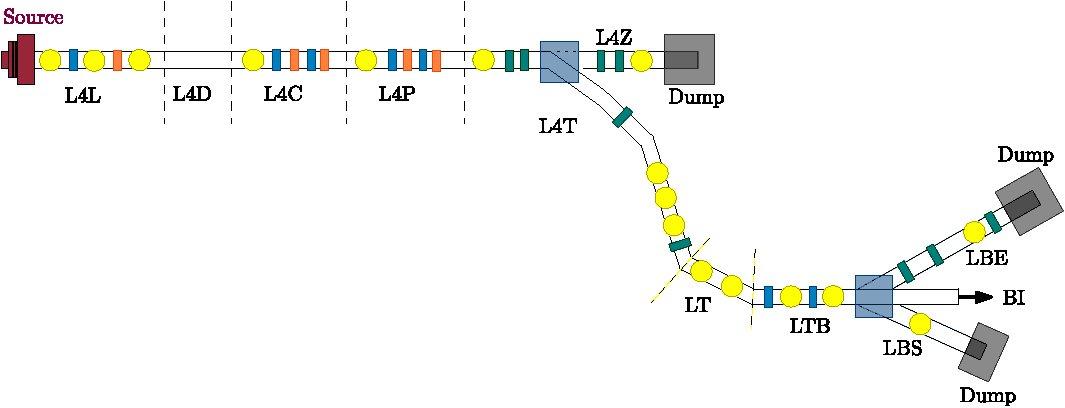
\includegraphics[width=1.0\columnwidth]{Linac4Instrumetnation/Linac4Instruments.pdf}
    \caption{Schematic representation of LINAC4 with the location of some diagnostics devices.}
    \label{fig:Linac4Layout}
\end{figure}

Figure \ref{fig:BCTwithTime} shows an example of intensity measurement taken by the first BCT in the L4T segment. From this figure, one can identify the beam pulse, we can observe that due to the accelerator of $H^{-}$ particles at LINAC4, the registered current is negative. In this case, the beam pulse length was 36 \si[]{\micro \second} with an average intensity of $\sim 17 $ \si[]{\milli \ampere}. One can observe the 1 \si[]{\micro \second} gaps generated by the chopper, which make the beam pulse ready to be injected into the different pulse rings. 

\begin{figure}
    \centering
    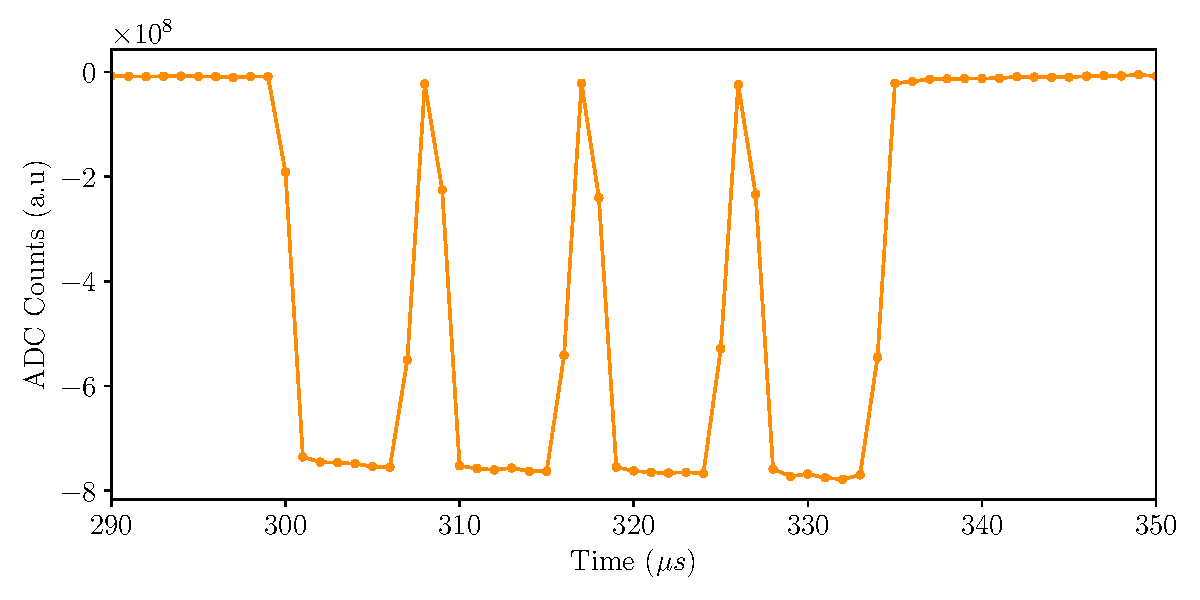
\includegraphics[width=0.7\columnwidth]{IntensityVStime/IntensityVStime.pdf}
    \caption[The LOF caption]{Beam current shape along beam pulse, from first BCT in L4T line.}
    \label{fig:BCTwithTime}
\end{figure}

By measuring the average current of the beam at all the available BCTs, one can assess the beam transmission along the accelerator. Figure \ref{fig:BeamTrans} shows an example of beam transmission measured along the accelerator. From this figure one can observe how in all parts of the accelerator, except for the first two BCTs in the L4L line, the current remains quite constant around $\sim 17$ \si[]{\milli \ampere}.  Similarly, the beam transmission remains very close to $100 \%$ along the whole accelerator. 

\begin{figure}
    \centering
    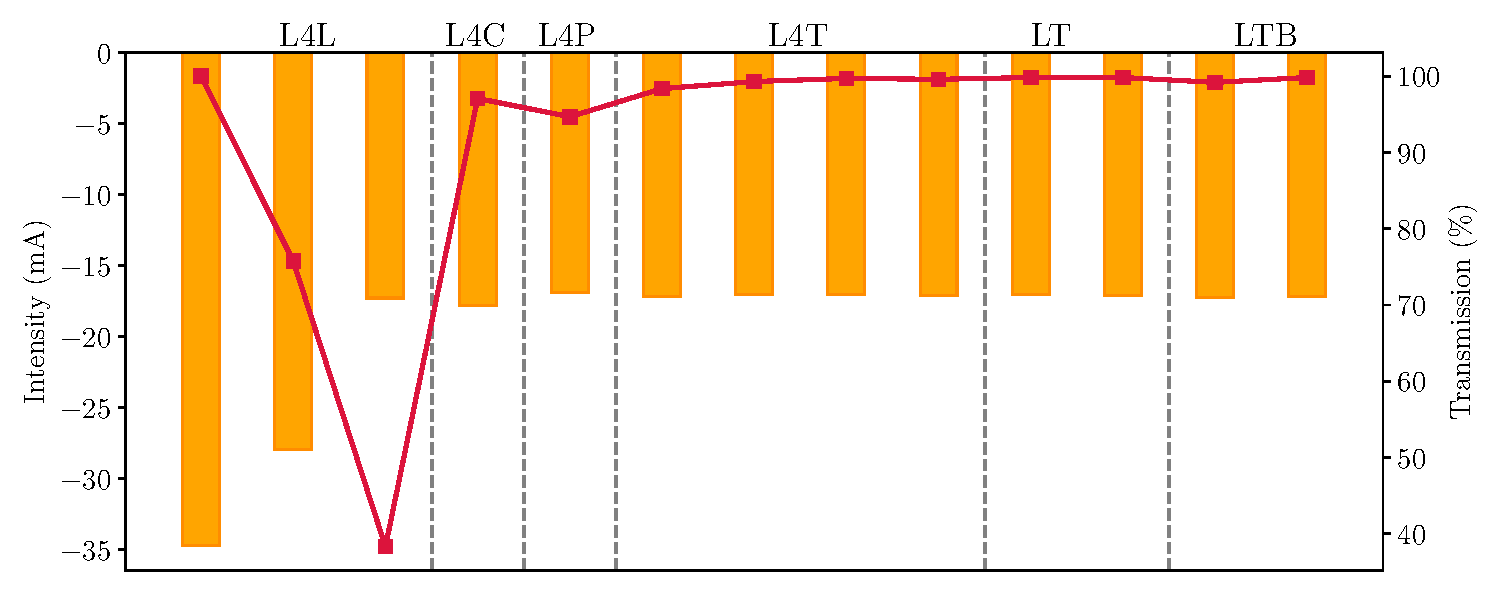
\includegraphics[width=0.9\columnwidth]{BCT_Transmission/TransmissionBCT.pdf}
    \caption{Average intensity measured by the different BCTs at LINAC4. Transmission along the LBE line.}
    \label{fig:BeamTrans}
\end{figure}


Similarly, the beam profile was measured along the accelerator, to cross-check the beam evolution as well as to assess the integrity and status of the devices installed along the accelerator.  Figure \ref{fig:HorizontalProf} shows the measurements of the horizontal profile of the beam along the LINAC4 accelerator. All these measurements were taken with the SEM grids. From this figure we can observe:

\begin{figure}
    \centering
    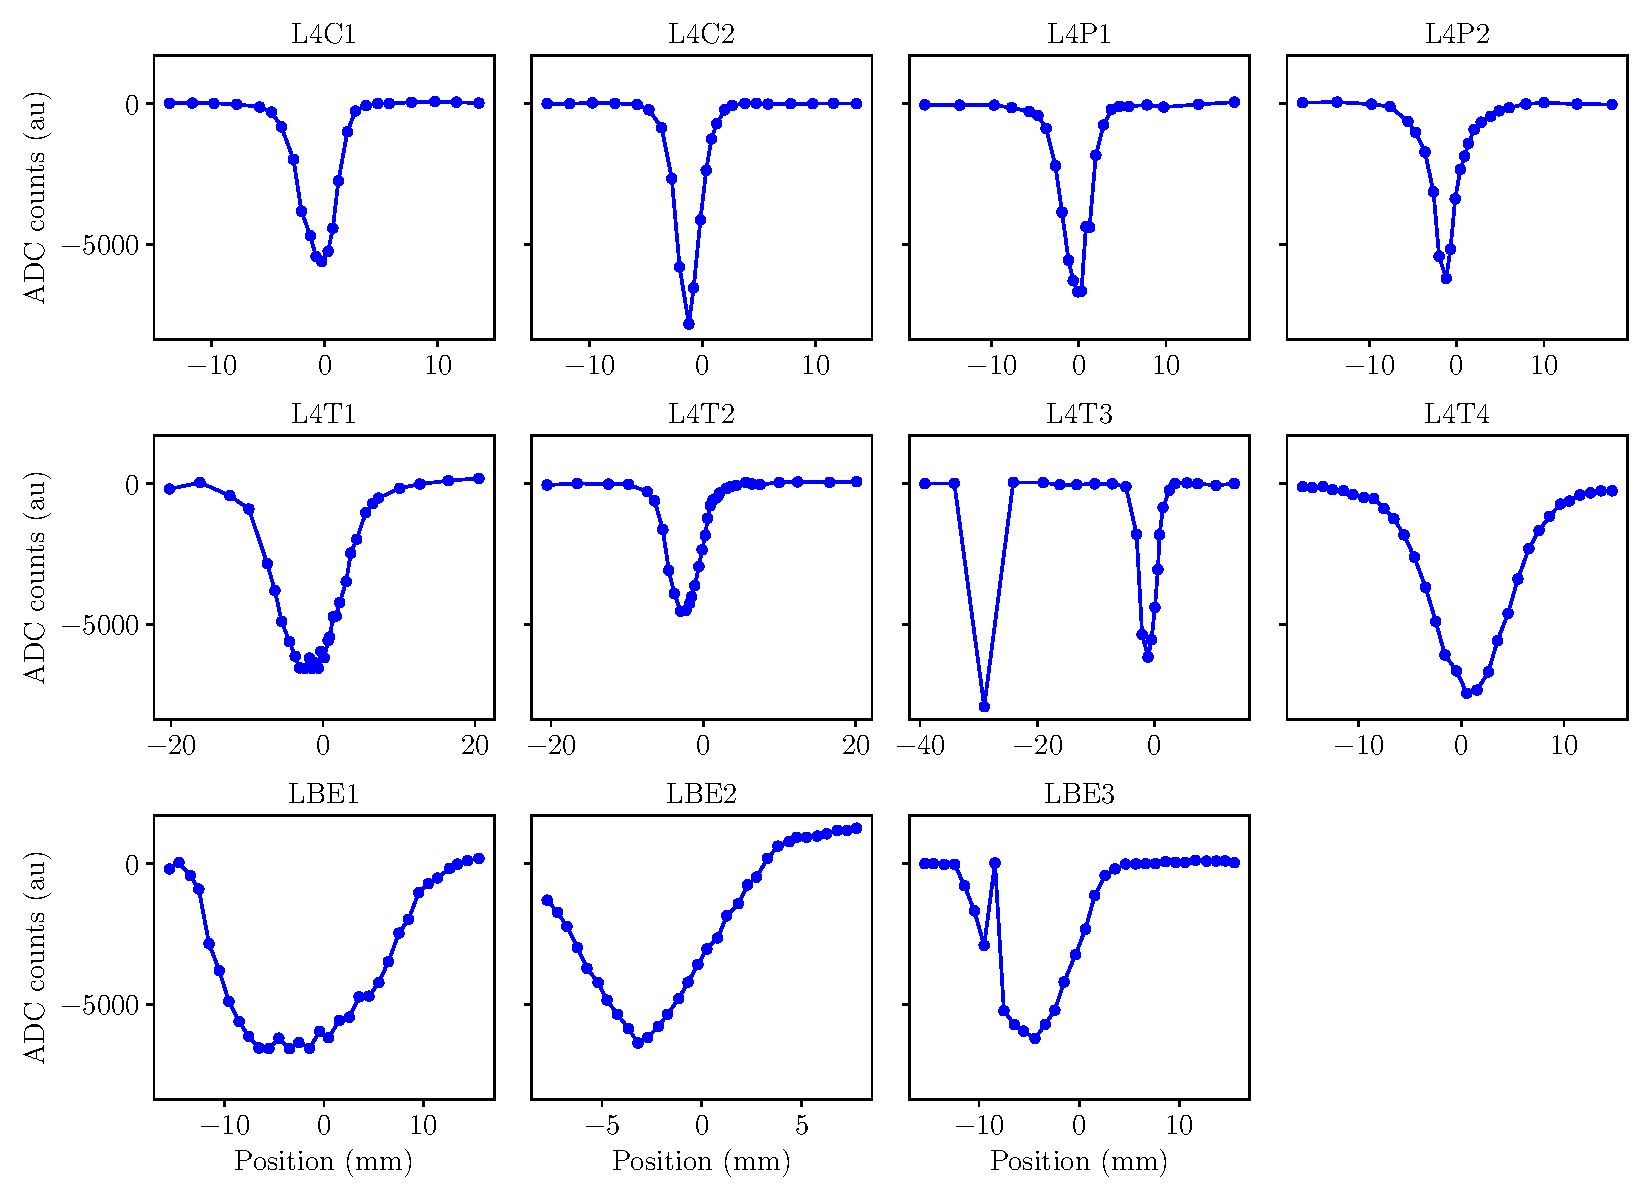
\includegraphics[width=1.0\columnwidth]{SigmaEvol/HorEvol.pdf}
    \caption{Horizontal transversal beam profile measured by the differt detectors at LINAC4}
    \label{fig:HorizontalProf}
\end{figure}

\begin{itemize}
    \item The beam profile seemed to be very much gaussian in all the measurement points except for LBE1 and LBE2 positions.
    \item Broken wires: SEM grids L4T2 and LBE3 present a broken wire that must be repaired. Wires 12-13 and 14-15 in L4P1 are glued together. 
    \item L4T1 and LBE1 present strange strange oscillations in the wires measuring the highest intensities. 
    \item Some of the grids have an even wire separation while others present a noneven wire distancing. Due to the beam not always being centered having smaller wire separation at the center of the grid des not seem to be that helpful.
    \item Not depicted, however, the data acquisition system for the detectors in the LBE sector had to be corrected to properly acquire the data.
\end{itemize}




Here we presented only the evolution of the horizontal profile, however, the evolution of the vertical profile was similarly studied. In the case of the vertical profile, a non-gaussian beam was observed in some of the locations. Figure \ref{fig:VertProf} shows an example of a vertical profile taken with both the second SEM grid and the second Wire Scanner from the L4T line. In this case, the particle beam clearly shows some shoulders or tails that push it away from the gaussian distribution. Another thing that one can observe from this figure, is the great agreement between the beam profile measurements by the sem grid and the wire scanner. 


These measurements were the first systematic set of measurements of the LBE run, they helped understand the beam evolution along the accelerator and thus helped correct the observed irregularities. These measurements also helped assess and correct any issue on the measuring devices, such as broken wires, position misreadings, data acquisition problems, etc.  

\begin{figure}[h]
    \centering
    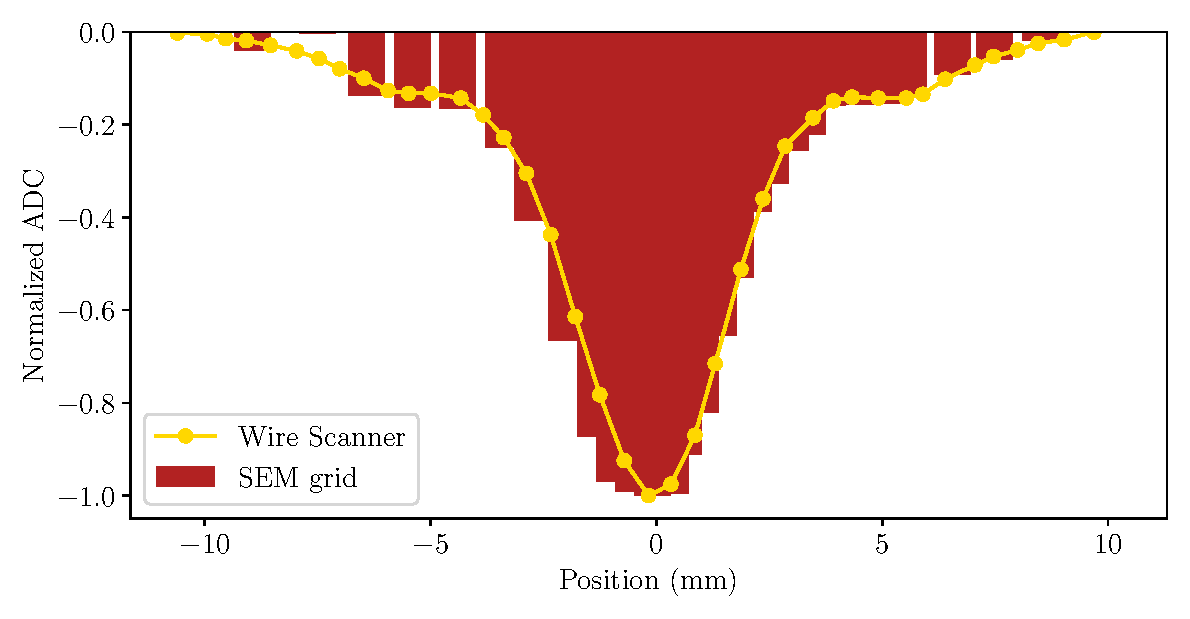
\includegraphics[width=0.6\columnwidth]{VertProf/VertProf.pdf}
    \caption{Vertical transverse profile measured by the second SEM grid and second wire scanner of the L4T line at Linac4.}
    \label{fig:VertProf}
\end{figure}






\chapter{Beam Matter Interaction} \label{ch:BeamMatterInter}
\pagestyle{fancy}

\graphicspath{ {Figures/Chapter3_BeamMatterInteraction/} }

The response characteristics of detection instruments employed during this desis depend on the interaction of charged particles with the sensitive elements of the detectors. In order to correctly interpret the measurements, it is fundamental to understand the various types of interactions between charged particles and matter. Many general reference works are available concerning this broad topic. For example, \parencite*[]{ref:Knoll}, \parencite*[]{ref:Evans} or \parencite*[]{ref:avernier} are very good references. This chapter will introduce only the theoretical concepts necessary for the comprehension of the latter chapters. 

\section{Particle matter interaction.}

The interactions that we will fixate on are primarily those related to Coulomb forces between the incident charged particle and the electrons and nuclei of the detector material. These include ionization, excitation, Bremsstrahlung and Cherenkov radiation. During these interactions, the incident charged particle loses its energy and it can be deflected from its original path. 

In the case of heavy charged particles, that is, particles whose rest mass is large compared with that of the atomic electron, inelastic collisions with atomic electrons are usually the predominant interaction mechanism. In such encounters, the electrons in the medium might experience a transition to an excited state (excitation) or to an unbound state (ionization). Since heavy particles are rarely deflected while traveling near an atomic nucleus, Bremsstrahlung production will be considered to be inconsequential. 

Cherenkov radiation will also be neglected as the conditions for its observation will never be reached in the casuistics of this thesis \parencite*[]{ref:Cherenkov}. For this reason, for the rest of the chapter, we will focus our attention solely to energy losses due to ionization and excitation processes. 

\section{Energy Loss: The Bethe Bloch Formula}
\label{sec:Bethe}

Stopping power is the parameter used to describe the gradual loss of energy of a charged particle as it penetrates into a medium. For a given heavy incident particle and target, this energy loss is very dependent on the particle velocity. In moderately relativistic energy ranges ($10$ - $10^6$ \si[]{\mega \electronvolt}/amu), the electrostatic stopping power is well defined by the Bethe Bloch theory \parencite[]{ref:Bethe}. 

\begin{equation}
    - \left< \frac{dE}{dx} \right> = Kz^2_e\frac{Z}{A}\frac{1}{\beta^2}\left[ \frac{1}{2} ln \left( \frac{2m_e c^2 \beta^2 \gamma^2 T_{max}}{I^2}\right) -\beta^2 - \frac{\delta\left(\beta \gamma\right)}{2} \right]
    \label{eq:bethe}
\end{equation}

With the symbol and parameter definitions given in table \ref{tab:ParBethe}. The units for the Stopping power are \si[]{\mega \electronvolt}/amu. The mean excitation energy is very dependent on the material, and it can vary from a few \si[]{\electronvolt} for materials with low Z to a hundred of \si[]{\electronvolt} for materials with high Z. A good approximation can be formulated as follows \parencite*[][]{ref:IonizationEne}:

\begin{equation}
    I \left[ eV \right] = 10 \cdot Z 
    \label{eq:ionizationEnergy}
\end{equation}

The maximum energy that can be transferred to a target electron in a single head-on collision is described by $T_{max}$, and can be approximated by the following formula \parencite*[][]{ref:TmaxFormula}: 

\begin{equation}
    T_{max} = \frac{2m_e c^2 \beta^2 \gamma^2}{1+\frac{\gamma m_e c^2}{M c^2}+\left( \frac{m_e c^2}{M c^2} \right)^2}
    \label{eq:tmax}
\end{equation}

Finally, $\delta (\beta \gamma)$ is a parametrized density correction factor necessary for highly relativistic particles \parencite*[][]{ref:Bethe}, its units are $MeV cm^2 g^{-1}$. It is important to notice that the energy deposited will very much depend on the characteristics of the incident particle as well as the absorber $\left( -\left< \frac{dE}{dx} \right> \propto \frac{Z}{A}  \right)$. 

\begin{table}[h!]
    \centering
    \begin{tabular}{ccc}
    \hline
    \textbf{Symbol}                  & \textbf{Definition}                  & \textbf{Units or Value}                                               \\ \hline
    $N_A$                      & Avogadro's Number           & $6.0221415(10)\cdot10^23$ $mol^{-1}$ \\
    $z_e$                      & Charge of incident particle &                                                              \\
    Z                       & Atomic number of absorber   &                                                              \\
    A                       & Mass Number of absorber     &                                                              \\
    I                       & Mean excitation energy      & eV                                                           \\
    $\beta \gamma$              & Relativistic parameters     &                                                              \\
    $m_e c^2$ & Electron Mass $\cdot$ $c^2$          & 0.510998918(44) MeV                                          \\
    $r_e$                      & Clasical Electron Radius    & 2.8179403250(28) fm                                          \\
    M                       & Incident Particle Mass      & $MeV/c^2$\\
    
    K/A                     & $4 \pi N_A r_e^2 m_e c^2/A$ & 0.307075 $MeV g^{-1} cm^2$  \\
     $\alpha$ & fine-structure constant & 1/137 \\ 
     \hline
    \end{tabular}
    \caption{Summary of variables used in this section.}
    \label{tab:ParBethe}
\end{table}


 Figure \ref{fig:EneDep} shows as an example, a comparison between energy deposition in thin target materials. In this particular case of thin target detectors, the energy deposition increases until reaching a maximum, after which it starts decreasing. From the image, we can observe that the energy deposited in graphite and copper is larger, due to their smaller mass number. Tungsten, gold and lead present smaller energy deposition values, and are similar to one another, due to their close atomic mass number. 

 \begin{figure}[h]
    \centering
    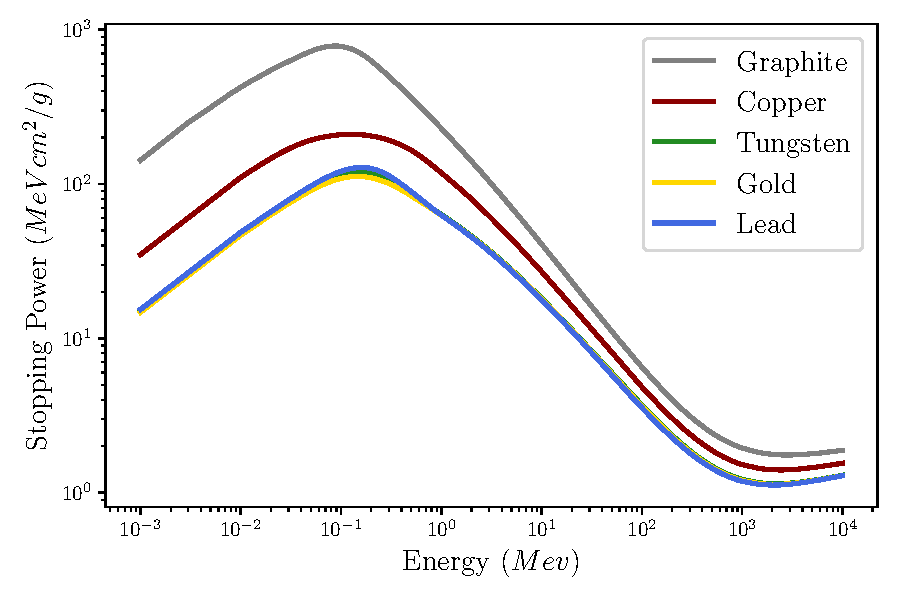
\includegraphics[width=0.7\columnwidth]{EdepMetal/EneDepMetal.pdf}
    \caption{Stopping powrer of protons in thin foils of different materials, as a function of incident particle energy. From \parencite*[][]{ref:NIST}.}
    \label{fig:EneDep}
\end{figure}

\section{Energy Loss in Mixtures and Compounds.}

As a first approximation, one can consider a compound to be made up of very thin layers of pure elements in the right proportion. That is: 

 \begin{equation}
    \frac{dE}{dx} =  \sum w_j \left.\frac{dE}{dx} \right\vert_j
 \end{equation}

Where $\left. \frac{dE}{dx}\right\vert_j$  is the energy loss in the j-th compound. However, it is important to remember that this is an approximation. The values of I and $\delta (\beta\gamma)$ are not perfectly represented by this addition method. More accurate values can be found in \parencite*[][]{ref:compound1} and \parencite*[][]{ref:compound2}, which include measured coefficients for nearly 200 mixtures and compounds. 

\section{Electrons Energy Loss}

For light particles such as electrons, bremsstrahlung losses are not negligible and can become dominant for energies above a few tens of \si[]{\mega\electronvolt}. One can define the critical energy $(E_c)$ as the point where the loss rates by Ionization and bremsstrahlung are the same \parencite*[][]{ref:EleCricEne}. 

\begin{equation}
    E_c = \frac{800}{Z + 1.2}
    \label{eq:ec}
\end{equation}

% When the energy of the incident particle is higher than the critical energy, one can define the energy loss by Bremsstrahlung as follows: 

% \begin{equation}
%     - \left< \frac{dE}{dx} \right> = \frac{E}{X_0}
%     \label{ref:edepElectron}
% \end{equation}

% With`$X_{0}$ being the radiation lenght, and defined as: 

% \begin{equation}
%     \frac{1}{X_0} = 4\alpha r^{2}_{e} n_{at} \left( Z^{2} \left[L_{rad}-f(Z)\right] + Z L^{'}_{rad}\right)
% \end{equation}

% \begin{equation}
%     L_{rad}(Z) = ln(184.15/Z^{1/3})
% \end{equation}

% \begin{equation}
%     L'_{rad} = ln (1194/Z^{2/3})
% \end{equation}

% Here, $n_at$ is the number of atoms per volume ($N_{av}\rho/A$). f(Z) is the coulomb correction function. 

Figure \ref{fig:BremssVSion} shows the stopping power of electrons in a thin tungsten target. From this figure we can see how in this case radiative losses become relevant after incident energies $\> 10 $\si[]{\mega\electronvolt}. This quantity is in agreement with equation \ref{eq:ec}.  

Due to the energy ranges and particles treated during this thesis, bremsstrahlung losses will not be considered as we will always remain under the critical energy regime. Some more information about how to model the energy losses due to this process can be found in \parencite*[][]{ref:BremstutorialG4}. 

\begin{figure}[h]
    \centering
    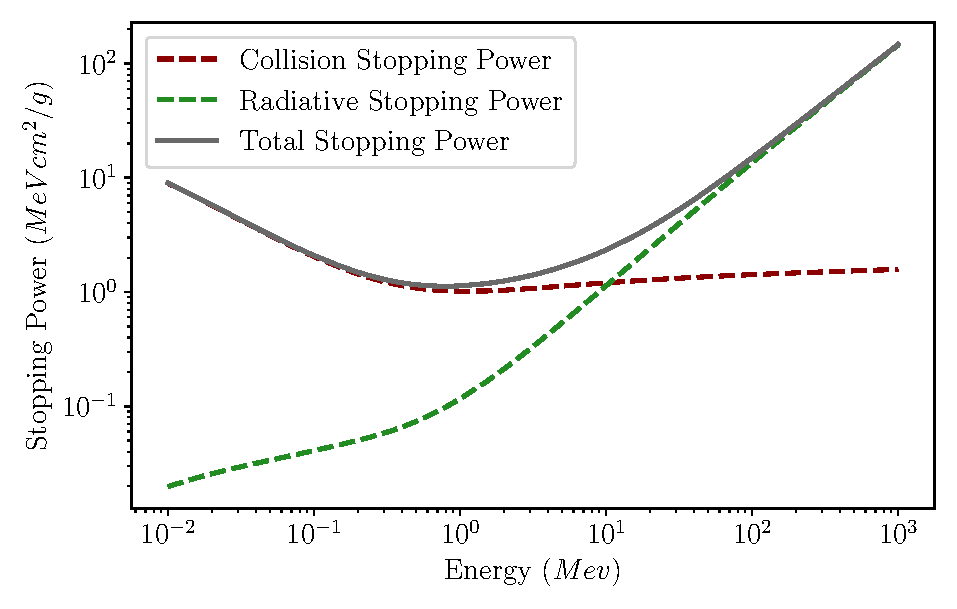
\includegraphics[width=0.7\columnwidth]{Electron_Edep/ElectronEdep.pdf}
    \caption{Stopping power of electrons in a thing tugsten foil, as a function of incident particle energy. From \parencite*[][]{ref:NIST}}
    \label{fig:BremssVSion}
\end{figure}

\section{Multiple scattering}

During the passage of the charged particle through the material, not only changes in the energy will occur, but also deflections from its original path. Most of these deflections occur due to Coulomb scattering with the atomic nucleus (Rutherford-type collisions). These collisions will result in small angular deflections ( if $m_{nucleus} >> m_{particle}$ ). Figure \ref{fig:PartScattering} shows a schematic representation of this process. 

\begin{figure}[h]
    \centering
    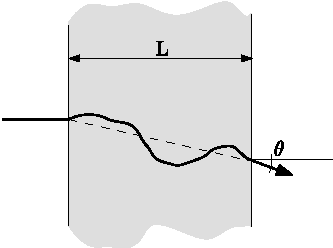
\includegraphics[width=0.4\columnwidth]{MultipleCoulombScat/MultipleScat.pdf}
    \caption{Schematic representation of multiple coulomb scattering.}
    \label{fig:PartScattering}
\end{figure}


The thicker the absorber and the larger its atomic number Z, the greater the likelihood that the incident particle will suffer multiple scatting events. Generally, 20 collisions are deemed sufficient to consider multiple scattering. For a sufficiently thick absorber, the mean number of successive encounters rises to a value that permits a statistical treatment of the problem. This is well represented by the theory of Moliere \parencite*[][]{ref:Moliere}, which assumes that after a distance L traveled through the material, the angular distribution of the particles with respect to their initial direction is Gaussian in shape and centered around the direction of the incident particles. This assumes that the deflection angle will be very small ($\theta \leq 10 \deg $). In these conditions, the mean square angle of such a Gaussian distribution can be calculated as follows: 


\begin{equation}
    \theta_0 = \frac{13.6 MeV}{\beta p c} z \sqrt{\frac{l}{X_0}}\left[ 1+0.038ln\left(\frac{l}{X_0}\right)\right] 
    \label{eq:multscat}
\end{equation}

Here $p,\beta c $ and z are the momentum, velocity and charge number of the incident particle and $l/X_0$ is the thickness of the medium measured in radiation lengths $X_0$, discussed in the following section. Experimental measurements show excellent agreement with the Gaussian distribution at small angles, and as expected, start differing at larger angles. This divergence can be explained due to the higher probability of close encounters which result in larger scattering angles. 

\section{Electron Back-Scattering}
\label{sec:BS}
It is very difficult to study any theory of multiple scattering for incident light particles such as electrons, due to the large number of scattering processes, not only by the atomic nuclei but also by the other electrons in the medium \parencite*[][]{ref:MultipleElec1} Equation \ref{eq:multscat} would need some corrections to properly describe the multiple scattering suffered by this light incident particle \parencite*[][]{ref:MultipleElec2}

\begin{figure}[h]
    \centering
    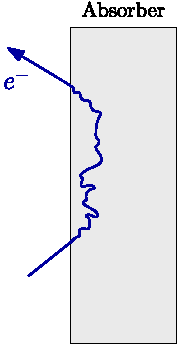
\includegraphics[width=0.25\columnwidth]{ElectronBS/ElectronBS.pdf}
    \caption{Back-scattering electron due to large multiple scattering angle.}
    \label{fig:backscatt}
\end{figure}

For light particles, large scattering angles are not rare. Those electrons that, after entering the material, are scattered back out are called backscattered electrons. See figure \ref{fig:backscatt} for a schematic representation of the phenomena.  Experimental information about this phenomenon has been intensively collected and from an empirical point of view, this phenomenon is well understood. On the other hand, attempts at a theoretical interpretation of the data have only limited success \parencite[][]{ref:BackScatTheo}.

For this document, we will only be concerned about the back-scattering electron yield ($BS_{el}$), which can be defined as the ratio between the number of outgoing primary electrons and the incident electron flux. Back-scattering of heavier particles, such as protos, is also possible. However, for our range of energies and material selection, we will consider this possibility to be negligible.


\section{Path Length and Range}
\label{sec:Range}
The distance traveled by a particle inside a target until it loses all its energy can be quantified by means of the range. The range is usually an experimental concept, and there are several definitions for it, but all of them relate roughly to the same quantity \parencite*[][]{ref:Knoll}. In this document, we will define the range (R) as the penetration depth in a medium that reduces the number of incident particles to one-half. The maximum penetration depth ($R_{max}$) is defined as the depth in the absorbing medium beyond which no particles are observed to penetrate. Finally, the total path length will measure the distance travelled by the particle measured along the actual path of the particle. Figure \ref{fig:RangeVsPathLength} illustrates the differences between these definitions. 

\begin{figure}[h]
    \centering
    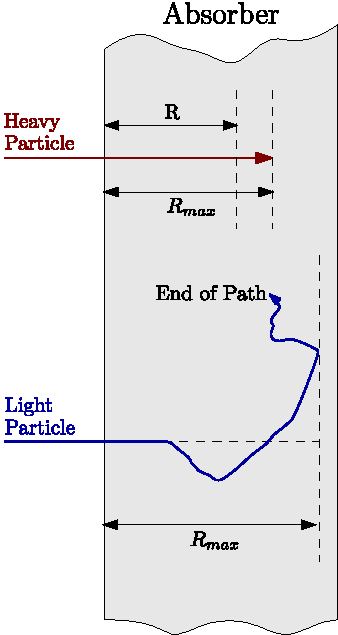
\includegraphics[width=0.30\columnwidth]{RangeVsPath/RangeVsPath.pdf}
    \caption{Schematic diagram of charged particle penetration into absorbing medium. Top: Heavy charged particle. Bottom: Light Charged particle.}
    \label{fig:RangeVsPathLength}
\end{figure}


The range highly depends on the type of particle, its initial energy and on the material through which it passes. Figure \ref{fig:RangeVsPathLength} also illustrates the differences between the path length and range of heavy and light particles. For a heavy particle that losses energy through ionization and atomic excitation, the range (R) can be calculated through the Continuous Slowing Down Approximation (CSDA). This approximation assumes a smooth path, without hard collisions and large-angle scattering. For a particle with an initial energy $E_0$, the CSDA range can be calculated as follows: 

\begin{equation}
    R_{CSDA} = \int_{0}^{E_0} \left( \frac{dE}{dx} \right)^{-1} dE
    \label{eq:rangeCSDA}
\end{equation}

Here the stopping power is considered to be a positive quantity. Some examples of analytical derivations of this equation can be found in \parencite*[][]{ref:CSDA}. The CSDA range for a heavy non-relativistic charged particles, of mass $M_0$ and energy $E_k$, in a given absorber can be written in terms of the proton CSDA range ($R^{p}_{CSDA}$)as follows: 

\begin{equation}
    R_{CSDA}^{M_0} \left( E_K \right)= \frac{1}{Z^2} \left(\frac{M_0}{m_p}\right) R_{CSDA}^{p}\left[ E_K \frac{m_p}{M_0}\right]
\end{equation}

Where $M_p$ is the proton mass and Z is the atomic number of the incident ion. This can be very useful, as the range of protons in a variety of absorbers has been extensively measured. For heavy charged particles, $R_{max} \sim R_{CSDA}$ in all types of absorbing media. 

In the case of light particles, this CSDA approximation is not valid due to the very tortuous path that they experience in the absorbing medium. In this case, the CSDA range can be up to twice the average path for high Z absorbers ($R_{max} = 1/2 R_{CSDA}$). A useful quantity in the case of light particles is called the radiation length ($X_0$), usually measured in $g cm^2$. This gives us a mean distance over which high-energy electron losses all but $1/e$ of its energy by Bremsstrahlung. Different approximations to this value are available in the literature, and each of them includes different degrees of approximations. Some of this expressions can be found in \parencite*[][]{ref:radiationLength}. Just as an example, this would be an expression for high energetic electrons in high Z materials: 

\begin{equation}
    X_0 = \frac{716.405 A}{Z\left(Z+1\right)ln\left(183 Z^{-1/3}\right)}
    \label{eq:radiationlength.}
\end{equation}

\section{Types of Absorbers}

In thin absorbers, only a few collisions of the projectile with the target atoms are likely to happen. Contrarily, in thick absorbers, a projectile makes many collisions and the projectile energy lost by the incident particle is considerable. One can consider a target to be thin when the range of the incident particles is much larger than the thickness of the material ($R(E_k) >> L$). For thin absorbers, the energy loss is small and the stopping power doesn't change much along the length of the material. In this case, the total energy loss in the absorber can be calculated as: 

\begin{equation}
    \Delta E = - \left(\frac{dE}{dx}\right)_{avg} \cdot L
    \label{eq:thinabs}
\end{equation}

In this case, the trajectory of the particle is also assumed to be perfectly linear in the absorber. If the range of the particles in the material is comparable to the thickness or smaller, this approximation is no longer valid, as one would underestimate the real energy deposition in the material. As the energy is lost, the probability of interactions with the absorber material increases as the ionization interaction cross-sections are bigger for smaller energies. The plot representing the specific energy loss along the incident particle track is called the Bragg curve. Figure \ref{fig:Bragg} shows an example of Bragg curve in the case of 3 \si[]{\mega\electronvolt} protons in graphite. 

\begin{figure}[h]
    \centering
    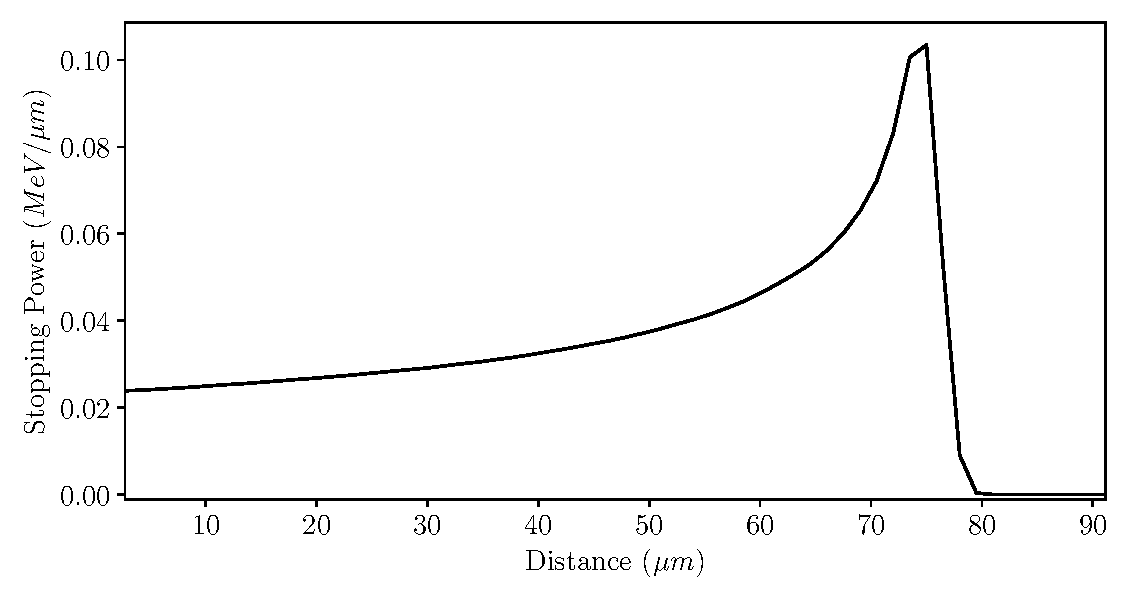
\includegraphics[width=0.7\columnwidth]{Bragg_Graphite/Bragg.pdf}
    \caption{Bragg peak of 3 \si[]{\mega \electronvolt} protons in Graphite. }
    \label{fig:Bragg}
\end{figure}

\section{Secondary Electron Theory}
\label{sec:SEY}
When a particle passes through the interface of a material, it will transfer energy to the
electrons in the medium. Depending on the energy these electrons get, they can be excited
to a higher energy level or gain enough energy to be emitted from the material, this emission
process is known as Secondary Electron Emission (SEE). The SEE phenomenon was already discovered in 1902 by Austin Starke \parencite*[][]{ref:see1} and it has been intensively studied since then. The SEE process can be generally divided into three consecutive steps:

\begin{enumerate}
    \item Generation Process: The minimum energy needed to create a Secondary Electron (SE) is the one required to ionize the atoms in the material. If the incident projectile is an ion containing electrons, these electrons can also be stripped off and produce further ionization. However, if the electrons from the incident ions are scattered off the material, they cannot be counted as secondary electrons. 
    \item Diffusion Process: While the SE travel through the material, they lose energy. This energy loss permits only a very shallow penetration depth of the low-energy electrons. For that reason, SE tends to be a surface phenomenon. 
    \item Emission Process: To be emitted from the surface, the SEs have to overcome the surface barrier potential \parencite*[][]{ref:see2}. The escape process is of particular importance because it determines the final shape of the secondary electron distribution. 
\end{enumerate}

\begin{figure}[h]
    \centering
    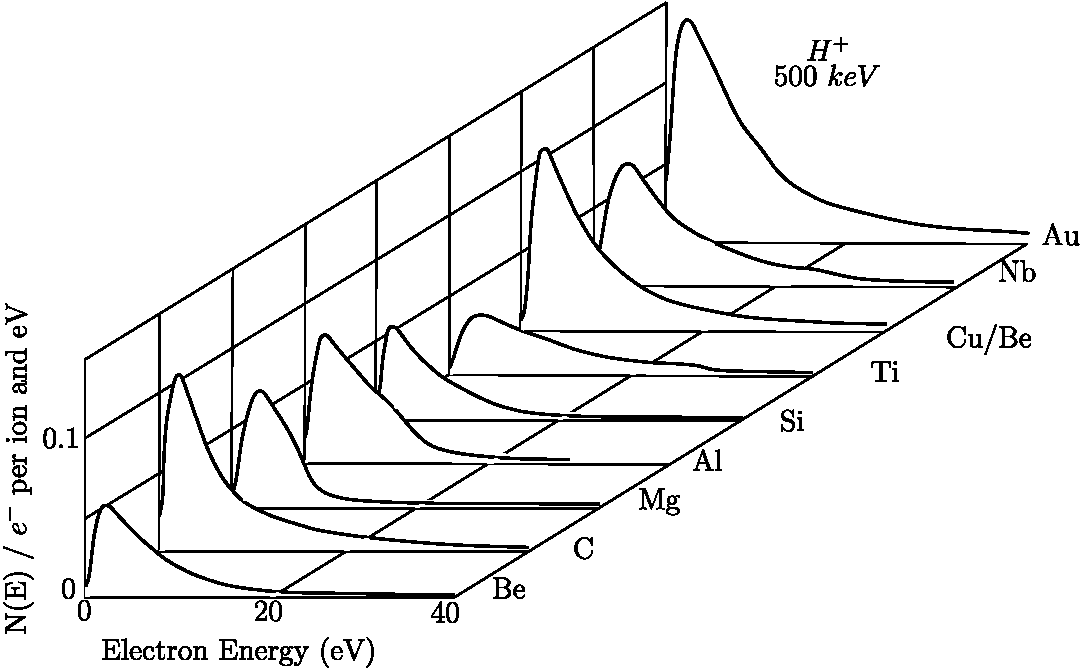
\includegraphics[width=0.9\columnwidth]{SEE_Spectra/SeeSpectra.pdf}
    \caption{Ion induced secondary electron spectra for a variety of metals. Incident ion: Proton 500 \si[]{\kilo \electronvolt}. From \parencite*[][]{ref:SEEspectra} }
    \label{fig:MetalsSE}
\end{figure}

Many experimental measurements on secondary electrons have been done since the discovery of this phenomenon, revealing some commonalities. In the case of SEE from metal surfaces \parencite*[][]{ref:see3},  The energy spectra of SEE peak at about 1-5 eV, showing a quick rise to the peak and then a slow reduction in the intensity. The full width of the peak is around 3-15 \si[]{\electronvolt}. At energies of several tens of \si[]{\electronvolt}, the intensity of the energy spectra is much weakened compared to the maximum peak. One can roughly say that the SE, in general, have an energy $< 50$ \si[]{\electronvolt}. Figure \ref{fig:MetalsSE} shows the spectra of SE emitted from different metals for an incident 500 \si[]{\kilo\electronvolt} proton. 

Not only SE must have an energy that allows them to escape the surface, but their velocity vector when reaching the surface must allow them to escape. In the case of metals and semiconductors, a cosine-type angular distribution of secondary electrons is observed \parencite[][]{ref:angleSemi}. 

The main parameter describing the SEE is the Secondary Emission Yield (SEY), which is the average number of electrons emitted per incident projectile. A semi-empirical treatment of SEY was formulated by E.J. Sternglass in 1957 \parencite*[][]{ref:SEY}. In this formulation, two sources of SE are considered. Firstly, the SE generated by small energy transfers from the incident particles to the target electrons. This first mechanism is the main contributor to the SEY. Secondly, a smaller contribution comes from the SE generated by delta electrons (which will be discussed in the following section). This formulation allows for the following numerical relation: 

\begin{equation}
    SEY = 0.01 L_S \left. \frac{dE}{dx}\right|_{el} \left[ 1+\frac{1}{1+5.4\cdot 10^{-6} E/A_p}\right]
    \label{eq:sey}
\end{equation}
\begin{equation}
    L_S = \left( 3.68\cdot 10^{-17} N_v Z^{1/3} \right)^{-1}
    \label{eq:LS}
\end{equation}

Here, E and $A_p$ are the kinetic energy and the mass of the projectile. Please notice that the electronic energy loss should be given in (\si[]{\electronvolt/\centi\metre}). $L_{s}$ is the characteristic length, which is of the order of the distance between inelastic collisions, and it is expressed in (\si[]{\centi\metre}). $N_v$ is the number of atoms per unit volume. The dependence of the incident particle energy comes with the term $dE/dx$. As we saw previously (\ref{sec:Bethe}), this term is greatly affected by the speed of the incident particle and its nature. 

The Secondary Emission Yield also depends on the angle of incidence of the incident particle. In the theory of Sternglass, the angular dependence is treated as a change in the effective penetration distance $L_{s}$. If the particle impacts under an angle different than normal, the effective track length of the projectile extends by a factor $1/cos(\theta)$. In that case the corresponding SEY would be: 

\begin{equation}
    \frac{SEY(\theta)}{SEY(0)} = \frac{1}{cos(\theta)}
\end{equation}

Experimental values confirm this approximation for incident angles up to $70\deg$. However, in the case of electrons as incident particles, recent measurements show a different angular dependence \parencite*[][]{ref:seyAngleEl}: 

\begin{equation}
    \frac{SEY(\theta)}{SEY(0)} = e^{0.5 \left(1-cos(\theta)\right)}
\end{equation}

Early investigations of SEE already show a dependence of SEE with temperature \parencite*[][]{ref:SeyVsTemp}. The temperature seems to affect the escape probability. An increase in temperature results in increased vibrations of the atoms about their equilibrium position which should reduce $L_{s}$, therefore increasing the Yield. Sternglass gives a rough quantitative hypothesis that goes as follows: 

\begin{equation}
    \frac{L_S (T_1)}{L_S(T_2)} = \frac{1+2.5\cdot 10^{-3}T_1}{1+2.5\cdot 10^{-3}T_2}
\end{equation}

It is important to note that the semiempirical theory of secondary emission is only considered to be accurate for backward emission (projectile entering the target). For the rear face of the target, the secondary emission is difficult to distinguish from the existing $\delta$ rays. On first approximation, we will also consider this formulation to be valid in the rear face assuming that the error due to $\delta$ raw emission can be neglected.  

\section{Delta Rays}

Most frequently, the electrons generated by SE have small energy. However, if the energy transferred to the electron is above a few hundred \si[]{\electronvolt} (up to $T_{max}$), they might be able to generate further ionization on their own. An analytical formulation for the total number of $\delta$-rays produced from charged particle interactions was presented by Rossi in 1952 \parencite*[][]{ref:delta1}, and gives the distribution of $\delta$ rays for incident particles with energy $I \ll T \ll T_{max}$ as follows: 

\begin{equation}
    \frac{d^2N_{\delta}}{dTdx} = \frac{1}{2}Kz^2\frac{Z}{A}\frac{1}{\beta^2}\frac{F(T)}{T^2}
    \label{eq:deltaN}
\end{equation}

Where $Tmax$ is given by equation \ref{eq:tmax}. The factor F is spin-dependent, but it is about unity for $ T \ll  T_{max}$. In order to calculate the total number of generated delta rays per unit of distance, one can integrate the previous equation from an arbitrary lower limit to the maximum energy delta rays can get ($T_{max}$). 






\label{ch:H0Hm}


% -------------- Include Appendixes ------------ %

%\appendix

\printbibliography 


\end{document}